\documentclass[12pt,a4paper]{report}

% ─── Packages ─────────────────────────────────────────────────────────────────
\usepackage[a4paper, left=1.5in, right=1in, top=1in, bottom=1in]{geometry}
\usepackage{graphicx}
\usepackage{hyperref}
\usepackage{fancyhdr}
\usepackage{titlesec}
\usepackage{tabularx}
\usepackage{setspace}
\usepackage{tocloft}
\usepackage{booktabs}
\usepackage{array}
\usepackage{ragged2e}
\usepackage{xcolor}
\usepackage{listings}
\usepackage{caption}
\usepackage{float}
\usepackage{times}
\usepackage{enumitem}
\usepackage{multirow}
\usepackage{makecell}
\usepackage{tabularx}
\usepackage{longtable}
\usepackage[nottoc]{tocbibind}
\usepackage{parskip}
\usepackage{array}
\usepackage[T1]{fontenc}
\usepackage{caption}
\captionsetup[lstlisting]{position=bottom}
\renewcommand{\arraystretch}{1.2}
\usepackage{listings}
\lstset{captionpos=b}

\usepackage{pifont}
\newcommand{\cmark}{\ding{51}}
\newcommand{\xmark}{\ding{55}}


% ─── Hyperref Setup ───────────────────────────────────────────────────────────
\hypersetup{
    colorlinks=true,
    linkcolor=black,
    urlcolor=blue,
    citecolor=black,
    pdftitle={ChatServe: Framework for WhatsApp-Based Small Business Automation},
    pdfauthor={Pravin Kanotara},
}

% ─── Spacing and Layout ───────────────────────────────────────────────────────
\onehalfspacing
\setlength{\parskip}{6pt}
\setlength{\parindent}{0pt}

% ─── Chapter and Section Formatting ──────────────────────────────────────────
\titleformat{\chapter}[display]
  {\normalfont\Large\bfseries\centering}
  {Chapter \thechapter}{10pt}{\LARGE}
\titlespacing*{\chapter}{0pt}{20pt}{30pt}

\titleformat{\section}{\large\bfseries}{\thesection}{1em}{}
\titleformat{\subsection}{\normalsize\bfseries}{\thesubsection}{1em}{}
\titleformat{\subsubsection}{\normalsize\bfseries\itshape}{\thesubsubsection}{1em}{}

% ─── Header / Footer ──────────────────────────────────────────────────────────
\pagestyle{fancy}
\fancyhf{}
\fancyhead[L]{\small\leftmark}
\fancyhead[R]{\small ChatServe}
\fancyfoot[C]{\thepage}
\renewcommand{\headrulewidth}{0.4pt}
\renewcommand{\footrulewidth}{0pt}

% ─── Code Listing Style ───────────────────────────────────────────────────────
\lstdefinestyle{codestyle}{
    backgroundcolor=\color{gray!8},
    commentstyle=\color{green!55!black},
    keywordstyle=\color{blue!80!black},
    numberstyle=\tiny\color{gray},
    stringstyle=\color{orange!80!black},
    basicstyle=\ttfamily\footnotesize,
    breaklines=true,
    keepspaces=true,
    numbers=left,
    numbersep=5pt,
    frame=single,
    rulecolor=\color{gray!40},
    tabsize=2,
}
\lstset{style=codestyle}

% ─── Custom Commands ──────────────────────────────────────────────────────────
\newcommand{\projecttitle}{ChatServe: A Framework for WhatsApp-Based Small Business Automation}
\newcommand{\studentname}{Pravin\ Kanotara}
\newcommand{\rollno}{22BCE139}
\newcommand{\guidename}{Prof.\ Monika Shah}
\newcommand{\hodname}{Dr.\ Ankit Thakkar}
\newcommand{\dept}{Computer Science and Engineering}
\newcommand{\university}{Nirma University}
\newcommand{\submityear}{April 2026}

% ══════════════════════════════════════════════════════════════════════════════
\begin{document}
% ══════════════════════════════════════════════════════════════════════════════

\pagenumbering{roman}

% ══════════════════════════════════════════════════════════════════════════════
% FRONT MATTER
% ══════════════════════════════════════════════════════════════════════════════

% ─── Title Page 1 — Simple Cover ─────────────────────────────────────────────
% TITLE PAGE

\thispagestyle{empty}
\begin{center}
{\huge ChatServe: A Framework for WhatsApp-Based Small Business Automation }\vspace{.05in}\\

\vspace{4cm}

Submitted By\\
{\large \bf Pravin Kanotara} \\
{\bf 22BCE139} \\
\vspace{4cm}

\begin{figure}[h]
\begin{center}
  
\includegraphics[scale=0.8]{Diagrams/Logo.jpg}
\end{center}
\end{figure}

{\bf DEPARTMENT OF COMPUTER SCIENCE AND ENGINEERING}\\
{\bf INSTITUTE OF TECHNOLOGY}\\
{\bf NIRMA UNIVERSITY}\\  
{\bf AHMEDABAD-382481}\\ ~\\ ~\\
{\bf April 2026}

\end{center}

% --------------------------------------------------------------------------------------------------------

\newpage
\thispagestyle{empty}
\begin{center}

{\huge ChatServe: A Framework for WhatsApp-Based Small Business Automation}\vspace{.05in}\\

\vspace{1cm}
{\large \bf Project Report}\\
\vspace{0.5cm}

{
Submitted in partial fulfillment of the requirements\\
\vspace{0.3cm}
for the degree of\\
\vspace{0.3cm}
\bf Bachelor of Technology in Computer Science and Engineering\\
}

\vspace{0.3cm} By\\
{\large \bf Pravin Kanotara} \\
{\bf (22BCE139)} \\
\vspace{0.4cm}

Guided By \\
{{\large\bf Prof. Monika Shah}} \\
\bf DEPARTMENT OF COMPUTER SCIENCE AND ENGINEERING\\

\vspace{3cm}
\begin{figure}[h]
\begin{center}
  
\includegraphics[scale=0.8]{Diagrams/Logo.jpg}
\end{center}
\end{figure}

{\bf DEPARTMENT OF COMPUTER SCIENCE AND ENGINEERING}\\
{\bf INSTITUTE OF TECHNOLOGY}\\
{\bf NIRMA UNIVERSITY}\\
{\bf AHMEDABAD-382481}\\ ~\\ ~\\
{\bf April 2026}

\end{center}




% ─── Certificate ─────────────────────────────────────────────────────────────
\newpage
\thispagestyle{empty}
\addcontentsline{toc}{chapter}{Certificate}
\begin{center}

\includegraphics[width=2.8in]{Diagrams/Logo.jpg}\\[1.2cm]
{\Large\textbf{Certificate}}\\[1.2cm]
\end{center}
\begin{center}
\begin{minipage}{0.99\textwidth}
\justifying
This is to certify that the project entitled \textbf{``\projecttitle''} submitted by \textbf{\studentname\ (\rollno)}, towards the partial fulfillment of the requirements for the award of the degree of Bachelor of Technology in \dept, \university, Ahmedabad, is the record of original work carried out by the candidate under our supervision and guidance. In our opinion, the submitted work has reached the level required for being accepted for examination.
\end{minipage}
\end{center}
\vspace{3cm}
\noindent
\begin{minipage}[t]{0.47\textwidth}
\textbf{\guidename}\\[0.3cm]
Assistant Professor\\
Department of \dept\\
Institute of Technology\\
\university, Ahmedabad
\end{minipage}
\hfill
\begin{minipage}[t]{0.47\textwidth}
\textbf{\hodname}\\[0.3cm]
Professor and I/C Head\\
Department of \dept\\
Institute of Technology\\
\university, Ahmedabad
\end{minipage}
\vspace{2cm}

% ─── Statement of Originality ────────────────────────────────────────────────
\newpage
\thispagestyle{empty}
\addcontentsline{toc}{chapter}{Statement of Originality}
\begin{center}
{\Large\textbf{Statement of Originality}}\\[0.5cm]
\hrule\vspace{1cm}
\end{center}
\begin{center}
\begin{minipage}{0.92\textwidth}
\justifying
I, \textbf{\studentname}, Roll No.\ \textbf{\rollno}, give an undertaking that the project entitled \textbf{``\projecttitle''} submitted by me towards the partial fulfillment of the requirements for the degree of Bachelor of Technology in \dept, \university, Ahmedabad, contains no material that has been awarded for any degree or diploma in any university or institution to the best of my knowledge.

This is original work carried out by me and I give assurance that no attempt of plagiarism has been made. It contains no material that is previously published or written, except where proper references have been made. I understand that any similarity found subsequently with published or dissertation work may result in severe disciplinary action.
\end{minipage}
\end{center}
\vspace{2.5cm}
\noindent\rule{5cm}{0.4pt}\\
Signature of Student\\[0.4cm]
\textbf{\studentname}\\
Roll No.: \rollno\\[0.5cm]
\vspace{2.5cm}
\begin{flushright}
Endorsed by\\[0.3cm]
\textbf{\guidename}\\
(Signature of Guide)
\end{flushright}

% ─── Acknowledgement ─────────────────────────────────────────────────────────
\newpage
\addcontentsline{toc}{chapter}{Acknowledgement}
\begin{center}{\Large\textbf{Acknowledgement}}\end{center}

I would like to express my sincere gratitude to my project guide, \textbf{\guidename}, for her continuous support, constructive feedback, and patient guidance throughout this project. Her insights helped shape both the technical direction and the academic framing of this work.

I am thankful to the \textbf{Department of Computer Science and Engineering, \university} for providing the infrastructure and the academic environment needed to carry out this project.

I would like to acknowledge \textbf{Meta Platforms, Inc.} for making the WhatsApp Cloud API accessible to developers and providing comprehensive documentation that served as the technical backbone of this system.

Finally, I am grateful to my family and friends whose encouragement kept me motivated throughout this journey.

\vspace{1.5cm}
\begin{flushright}
\textbf{\studentname}\\
\textbf{\rollno}\\
\end{flushright}

% ─── Abstract ────────────────────────────────────────────────────────────────
\newpage
\addcontentsline{toc}{chapter}{Abstract}
\begin{center}
{\Large\textbf{Abstract}}
\end{center}
\vspace{1em}

This project presents the development of a web-based framework designed to support small-scale, home-based, and seasonal businesses in managing their operations efficiently. Although platforms like WhatsApp Business are commonly used for customer communication, they lack structured features for handling orders, service bookings, and data management.
The proposed system follows a hybrid model, where business owners manage products, services, and customer data through a web application dashboard, while customers interact via WhatsApp. A chatbot-based interface is integrated to assist customers by responding to queries, displaying product or service information, enabling order placement or booking, and providing status updates.
This approach combines the simplicity of chat-based communication with the efficiency of a structured backend system. The solution is designed to be user-friendly, lightweight, and accessible, helping small businesses improve customer experience, streamline operations, and adopt digital tools with minimal technical complexity.

% ────────────────────
\newpage
\tableofcontents

\newpage
\listoffigures

\newpage
\listoftables

% ══════════════════════════════════════════════════════════════════════════════
% CHAPTERS
% ══════════════════════════════════════════════════════════════════════════════
\newpage
\pagenumbering{arabic}
\setcounter{page}{1}

% ══════════════════════════════════════════════════════════════════════════════
% CHAPTER 1 — PROBLEM CONTEXT AND MOTIVATION
% ══════════════════════════════════════════════════════════════════════════════

\chapter{Problem Context and Motivation}

\section{Background of MSME and Informal Sector}

India is home to the largest MSME community in the world and that has been very integral in fueling the economy. In the order of 6.5 crore (65 million) MSMEs are present at the moment over the country and they also put out almost 30.1\% of our national GDP, 35.4\% of the manufacturing output and 45.73\% of what we export. Also we have near 28 crore people employed in this area, which is a large part of the work force \cite{pib_msme2025}. In that large sphere small businesses and service providers are a big segment. We have home-based businesses, local shops, salons, freelancers, cloud kitchens we have them all. These are very much a part of urban and semi urban life, and a lot of people depend on them daily.

The owners lack the technical skill, also they do not have time to spare, and they would rather not pay for the expensive digital tools.

Now in India WhatsApp is very popular. We see a user base of over 500 million which is reported in \cite{hyperleap_india2026}. It has in fact become the primary communication platform for large sections of small businesses. Owners use it for taking orders, sharing product or service catalogs, replying to questions and in general staying in touch with customers. But the standard WhatsApp Business App is a little out of date. While it does basic messaging very well it does not have in it the automated features which a proper order and booking management system would require.

% ─────────────────────────────────────────────────────────────────────────────

\section{Real-World Observations}

In a look at how small businesses run their day to day ops WhatsApp is what they use the most. The owner goes through each message, looks at availability, does the math and either notes it in a notebook or does it in her head. That is the main routine for most. When it is busy during peak hours for example -- that break down. At the same time multiple customers are messaging in at which point the owner just can't keep up. Orders go out the window, responses are delayed, and details are left out. WhatsApp is for chat not business which is why it does not have in it any order tracking, auto response, or structuring of workflow.

Many of these business owners do not have low-cost tools that could help them manage their businesses. The available tools either require too much technical knowledge for the owner to understand how to use them or involve such high recurring subscription costs that they are not feasible for small businesses that are often tight on cash and can't afford to pay for them.

All of this indicates that there is clearly a demand for a solution that is straightforward and easy to use, allows users to seamlessly integrate into WhatsApp, and can automate the repetitive steps of collecting orders and bookings so that these businesses can spend time on the other important tasks in their business. Enhancing productivity and improving the customer experience through streamlining the ordering and booking process will have a significant impact on the way they work with their customers.

% ─────────────────────────────────────────────────────────────────────────────

\section{Problem Statement}

In India, the small business sector relies heavily on WhatsApp to communicate and manage their order processes and communications with customers; however, small businesses don't have affordable, easy-to-utilize tools capable of automating any part of this very important set of tasks. The tools available today are all very much at two different ends of the spectrum: on one side is the no-cost WhatsApp Business App which only allows for basic messaging (with no ability to provide additional functionality to help engage customers); on the other side is an API-based platform that provides many advanced features including automated responses and analytics to help engage customers, but these solutions are often too expensive to implement and require extensive technical expertise for implementation and ongoing support.

Limited availability in their capacity to easily access tools creates a scenario whereby the majority of micro/small businesses find themselves reliant on manual processes to complete their operations. Consequently, many micro/small businesses suffer from operational challenges associated with the reliance on manual processes, such as missed orders, slow response times to customer inquiries, and a lack of visibility into the one's overall performance and operational efficiency level. The result is a significant gap in the market as these small businesses have no way to compete effectively in an increasingly fast-paced digital world due to the lack of reasonably priced user-friendly solutions that specifically address their unique needs.

The core question we're trying to answer is: \textit{How can a small business owner access automated WhatsApp-based order and booking management without technical knowledge, without significant cost, and without complex setup requirements?}

\begin{table}[htbp]
    \centering
    \small
    \begin{tabular}{|p{3.5cm}|c|c|p{3cm}|}
        \hline
        \textbf{Business Size} & 
        \textbf{\shortstack{WhatsApp \\ Business App}} & 
        \textbf{\shortstack{WhatsApp \\ Business API}} & 
        \textbf{Reason} \\
        \hline
        \shortstack[l]{Micro \\ (1--5 emp.)} & 92\% & 2\% & Cost, simple \\
        \hline
        \shortstack[l]{Small \\ (6--25 emp.)} & 75\% & 15\% & Basic automation \\
        \hline
        \shortstack[l]{Medium \\ (26--200 emp.)} & 40\% & 55\% & Multi-user, integration \\
        \hline
        \shortstack[l]{Large \\ (200+ emp.)} & 10\% & 85\% & Scale, CRM sync \\
        \hline
    \end{tabular}

    \vspace{0.2cm}
    \caption{WhatsApp Business Adoption by Enterprise Size in India \cite{hyperleap_india2026}}
    \label{tab:adoption_by_size}
\end{table}

% ─────────────────────────────────────────────────────────────────────────────

\section{Objectives of the Study}

What we have put forth with this project is very simple -- we are to develop a system which enables small business owners to use WhatsApp for their order and booking management which in turn they do not have to get into the technical aspects of. As for the main goals they are:.

\begin{enumerate}

    \item To create a conversational onboarding experience which is technical knowledge free for business owners. 
    \item To put in place an automated order and booking handling via a WhatsApp based chatbot. \item To present a very simple and intuitive interface for managing product/service catalogs and orders. 
    \item To put forward a scalable system architecture for many businesses (multi-tenant SaaS model). 
    \item To keep the overall system affordable and simple enough that small businesses can actually get it running without much hassle.

\end{enumerate}.


% ─────────────────────────────────────────────────────────────────────────────

\section{Scope of the Project}

This project which has put forth a WhatsApp based automation system for small businesses. We do chatbot which takes care of order and booking processing, a business owner's on boarding guide and also a web dashboard for day to day management. Although we have designed the system with the Indian MSME sector in mind, the base structure of the system is flexible enough to be used by various types of small scale businesses including home-based ventures, salons, local shops, and freelancers. To that effect we have excluded a few elements from the present scope:.

\begin{itemize}

\item Integration with external payment gateways

\item Multi-language chatbot support

\item Delivery partner integration

\item Advanced analytics and reporting features

\end{itemize}    % Chapter 1 — Problem Context and Motivation
% ══════════════════════════════════════════════════════════════════════════════
% CHAPTER 2 — LITERATURE REVIEW (FINAL CLEAN VERSION)
% ══════════════════════════════════════════════════════════════════════════════
\chapter{Literature Review}

\section{MSME Landscape and Statistical Analysis}

The MSME sector is a very key component of India's economy. It puts out around 30.1\% of the national GDP which is a very large number. Also it accounts for almost 35.4\% of what we see in manufacturing output and also about 45.73\% of total exports. We have in India around 6.5 crore registered MSME units and these businesses together put to work almost 28 crore people as of \cite{pib_msme2025}. In terms of scale and impact it is safe to say that this sector is very at the core of the Indian economy.

One to note is the rate at which formalization is taking off. By April 2026 we saw registration of about 7.94 crore enterprises via the Udyam Registration and the Udyam Support Platform (UAP). That is a large scale increase and it is a sign that we are seeing greater recognition and integration of small scale businesses into the main economic structure \cite{msme_annual_report}. \begin{table}[htbp].

\centering

\small

\begin{tabular}{|l|r|}

\hline

\textbf{Category} & \textbf{Number of Enterprises} \\

\hline

Total MSMEs & 7,94,25,711 \\

Udyam Registered & 4,72,77,069 \\

UAP Registered & 3,21,48,642 \\

\hline

\end{tabular}

\caption{MSME Registration Statistics \cite{msme_annual_report}}

\end{table}

If you take a closer look at the distribution you'll see what I mean in that field we have almost only micro enterprises.


\begin{table}[htbp]
\centering
\small
\begin{tabular}{|l|r|}
\hline
\textbf{Enterprise Type} & \textbf{Count} \\
\hline
Micro Enterprises & 7,88,97,394 \\
Small Enterprises & 4,91,260 \\
Medium Enterprises & 37,057 \\
\hline
\end{tabular}
\caption{MSME Distribution by Enterprise Category \cite{msme_annual_report}}
\end{table}

What we see is that by and large the preponderance of businesses in India are very small. They work with limited resources and also for the most part do not have much in terms of technology infrastructure. Although we see high adoption of smart phones by business owners today what they do with technology is still very basic. It is mostly for communication and may also include digital payments not for the running of the business like order tracking, customer management, or inventory. In large part those functions are still performed manually.

In the MSME sector we see that it is micro and small businesses which use what they are familiar with, what is everyday to them. There is a true need for basic digital solutions which may help them to work better without at the same time requiring them to become tech savvy over night.

% ─────────────────────────────────────────────────────────────────────────────

\section{Informal Business Characteristics}

In India a large number of MSMEs operate in the informal sector which include small scale and home based businesses. These businesses are mostly run by a single individual or a family, have low investment, a small work force and do not have formal digital systems. Because of their informal structure these companies use mainly manual processes which include hand written notes and direct messages for order and booking management. In this segment technology adoption is very much dependent on how simple and familiar the system is. Companies do not adopt complex set up or technical tools which require great IT skill, instead they prefer tools that fit into their present work flow.

% ─────────────────────────────────────────────────────────────────────────────

\section{Adoption of WhatsApp in Small Businesses}

WhatsApp has become a global leader in terms of which communication platform is used, with over 2 billion monthly active users. In India it is the largest digital communication player, with a reported user base of over 530 million which we may assume to be nearly all smartphone users there \cite{hyperleap_india2026}. We see that daily on the platform there are over 100 billion messages sent out which speaks to the scale and reliability of the platform \cite{infobip_stats2026}. Also in the area of business communication we see very high adoption. Over 200 million businesses world wide use WhatsApp Business accounts and also a large number of small and medium sized businesses use it for every day customer communication \cite{infobip_stats2026}. Also we see that over 175 million users are interacting with businesses daily on WhatsApp which plays a large role in customer engagement \cite{d7_stats2026}.

WhatsApp reports to have very high engagement numbers. We see open rates of up to 98\% for business messages and also that they get much better response rates which is a great improvement over what we see in traditional communication methods like email and SMS.

\begin{table}[htbp]
    \centering
    \begin{tabular}{lccc}
        \hline
        \textbf{Metric} & \textbf{WhatsApp} & \textbf{Email} & \textbf{SMS} \\
        \hline
        Open Rate & 98\% & 22\% & 95\% \\
        Response Rate & 45\% & 6\% & 12\% \\
        Click-through Rate & 35\% & 3\% & 8\% \\
        Conversion Rate & 15\% & 2\% & 4\% \\
        \hline
    \end{tabular}
    \vspace{0.2cm}
    \caption{Engagement Comparison: WhatsApp vs. Traditional Channels \cite{hyperleap_india2026}}
    \label{tab:engagement_stats}
\end{table}

These engagement numbers prove that which WhatsApp has become the go to platform for business communication. We see that our users are on the app daily which in turn makes it very effective for real time communication and order management.

% ─────────────────────────────────────────────────────────────────────────────

\section{Challenges Identified in Existing Practices}

Despite wide scale adoption most MSMEs are still using WhatsApp in a very unstructured and manual way. Business owners use the single chat interface for customer service, order info, and payments which in turn causes issues and increases their work load. Also we see that customer expectations have grown. Immediacy is what makes the platform successful we see that the large majority of messages are read very quickly. We also note that consumers expect prompt response; many expect reply within an hour and they will take their business elsewhere if they don't get it which is reported in \cite{hyperleap_india2026}. This puts great pressure on small business owners who are trying to manage many conversations at once without support of automation.

While in the case of WhatsApp Business API which provides chatbots, multi agent support, and CRM integration they do so at a high cost and also from a technical point of view it is a complex solution. Also these platforms require business to go through a verification process, API integration, and system configuration which in turn makes them a no go for what we term as informal and small scale businesses. Thus we see that adoption of what may be classified as advanced automation features is very low in micro businesses.

This creates a clear gap use of WhatsApp and lack of accessible automation tools for MSMEs. Addressing this gap forms the foundation for the proposed ChatServe system.  % Chapter 2 — Literature Review
% ══════════════════════════════════════════════════════════════════════════════
% CHAPTER 3 — EXISTING SYSTEM AND GAP ANALYSIS (FINAL)
% ══════════════════════════════════════════════════════════════════════════════

\chapter{Existing Systems and Gap Analysis}

% ─────────────────────────────────────────────────────────────────────────────

\section{Requirements of MSMEs and Small Enterprises}

Small enterprises and informal setups, particularly in service-oriented and product-based sectors, operate in high speed and require constant interactions with the customers. For such organizations, ease-of-use and affordable solutions are required.

Requirements of MSMEs:
\begin{itemize}
    \item Simplified interface
    \item Order and booking handling with automation
    \item Real time communication
    \item Order, booking, and customer centralization
    \item Cost-effective solutions
    \item Scalability
\end{itemize}

But current solutions do not cater to all of the above requirements.

% ─────────────────────────────────────────────────────────────────────────────

\section{WhatsApp Based Existing Solutions}

\subsection{WhatsApp and WhatsApp Business App}

WhatsApp and WhatsApp Business apps are the two popular options adopted by small organizations due to simplicity and ease-of-access.

\textbf{Facilities Provided:}
\begin{itemize}
    \item Messaging and file sharing
    \item Profile setting and products catalog
    \item Reply and label management
    \item Away messages
    \item Broadcast messages and status updates
\end{itemize}

\textbf{Drawbacks:}
\begin{itemize}
    \item Lack of any automation facility
    \item Lack of multi-user access
    \item Lacks any analytics tools
    \item Complete manual operations
\end{itemize}

% ─────────────────────────────────────────────────────────────────────────────

\subsection{WhatsApp Business API Based Platforms}

The platforms overcoming the above issues provide automation and other advanced features.

\textbf{General Facilities in All Platforms:}
\begin{itemize}
    \item Chatbot for automation
    \item Multi-agents access
    \item Campaigns and notifications
    \item CRM integration and handling
    \item Integration to other systems
    \item Reporting and analytics
\end{itemize}

% ─────────────────────────────────────────────────────────────────────────────

\section{Platform-wise Analysis}

\subsection{Interakt}

Interakt is a conversation management and CRM system using WhatsApp for small and medium organizations.

\textbf{Facilities provided:}
\begin{itemize}
    \item Agent access through shared inbox
    \item Automation and auto replies
    \item Basic AI for FAQs and lead handling
    \item Product catalog
    \item Broadcasting
    \item Integrations with Shopify and WooCommerce
    \item Reporting
\end{itemize}

\textbf{Strengths:}
\begin{itemize}
    \item Easy to use
    \item Cost effective for small organizations
    \item User-friendly
\end{itemize}

\textbf{Weaknesses:}
\begin{itemize}
    \item Less advance analytics
    \item Moderate scalability
    \item Basic AI facility
\end{itemize}

% ─────────────────────────────────────────────────────────────────────────────

\subsection{AiSensy}

It is an automated WhatsApp marketing platform designed for campaigns and customer interaction.

\textbf{Facilities provided:}
\begin{itemize}
    \item Broadcast campaign and segmentation
    \item Bot creator with no coding
    \item Click to WhatsApp for advertising
    \item CRM and contact segmentation
    \item Campaign analytics and reporting
    \item Message template
    \item AI based analysis
\end{itemize}

\textbf{Strengths:}
\begin{itemize}
    \item Good for marketing
    \item Cost effective
    \item Ease of use
\end{itemize}

\textbf{Weaknesses:}
\begin{itemize}
    \item Limited omnichannel capabilities
    \item Limited customization
    \item Limited AI facilities
\end{itemize}

% ─────────────────────────────────────────────────────────────────────────────

\subsection{WATI}

It is a customer communication platform with WhatsApp for small and medium organizations.

\textbf{Facilities provided:}
\begin{itemize}
    \item Agent access through shared inbox
    \item Chatbot creation with no code
    \item Broadcasting
    \item Segmentation of the contacts
    \item Integrations with CRMs
    \item Basic dashboards
    \item Workflow management
\end{itemize}

\textbf{Strengths:}
\begin{itemize}
    \item Easy to onboard and use
    \item Efficient for customer support processes
\end{itemize}

\textbf{Weaknesses:}
\begin{itemize}
    \item Limited analytics
    \item Moderate scalability
    \item Basic AI tools
\end{itemize}

% ─────────────────────────────────────────────────────────────────────────────

\subsection{Infobip}

It is a business communication platform providing omnichannel communication.

\textbf{Facilities Provided:}
\begin{itemize}
    \item Omnichannel communication using WhatsApp, SMS, and emails
    \item Advanced AI chatbot
    \item Customer journey automation
    \item Real time analytics and reporting
    \item API integration
    \item Campaign automation
    \item Security
\end{itemize}

\textbf{Strengths:}
\begin{itemize}
    \item Highly scalable
    \item Advance automation and analytics
    \item Omnichannel support
\end{itemize}

\textbf{Weaknesses:}
\begin{itemize}
    \item Expensive to use for small businesses
    \item Complex setup and management
    \item Inappropriate for MSMEs
\end{itemize}

% ─────────────────────────────────────────────────────────────────────────────

\section{Comparison Between the Platforms}

\begin{table}[htbp]
\centering
\scriptsize
\renewcommand{\arraystretch}{1.3}

\begin{tabularx}{\textwidth}{|p{2.5cm}|X|X|X|X|X|X|}
\hline
\textbf{Feature} & \textbf{WA Business} & \textbf{Interakt} & \textbf{AiSensy} & \textbf{WATI} & \textbf{Infobip} & \textbf{Respond.io} \\
\hline
Automation & Basic auto replies & Workflow automation & Campaign automation & Chatbot automation & Advance automation & Flow automation \\
\hline
Bot & Not available & Basic bot & Rule-based bots & Bot creation & AI bots & AI agents \\
\hline
Multi-user & Not possible & Multi-agent & Multi-agent & Multi-agents & Enterprise & Omnichannel \\
\hline
Analytics & Limited analytics & Campaign analytics & Marketing analytics & Analytical dashboard & Advanced analytics & Detailed reports \\
\hline
AI features & Not available & Basic AI facility & AI tools & Limited AI & Advance AI facility & AI agents \\
\hline
Marketing & Only broadcast messages & Campaigns & Campaigns and advertising & Limited advertising & Full automation & Re-engagement \\
\hline
Channel Supported & WhatsApp only & WhatsApp and Instagram & WhatsApp only & WhatsApp & Omnichannel & Omnichannel \\
\hline
Pricing & Free & ₹2,499/month & ₹1,500/month & ₹1,999/month & Enterprise level & \$79/month+ \\
\hline
Trial period & Not available & 14 days trial & Trial + Free account & 7 days trial & No trial & 7 days trial \\
\hline
Ease of Use & Very easy & Easy & Easy & Moderate & Difficult & Moderate \\
\hline
Setup effort & None & Low effort & Low effort & Moderate effort & High effort & Moderate effort \\
\hline
Scalability & Not scalable & Medium scalability & Medium scalability & Medium scalability & Highly scalable & Highly scalable \\
\hline
\end{tabularx}

\caption{WhatsApp Business Platforms Comparison \cite{whatsapp_difference}}
\end{table}

% ─────────────────────────────────────────────────────────────────────────────

\section{Limitations of Current Solutions}

\begin{itemize}
    \item High price for complex platforms
    \item Technical complexities in setup and usage
    \item Interface difficulties for non-technical persons
    \item Complexity of unnecessary features
\end{itemize}

% ─────────────────────────────────────────────────────────────────────────────

\section{Identifying Research Gaps}

Current approaches provide ease of use but do not include any automated process, while those that are automated are difficult and costly.

The following characteristics cannot be combined successfully:
1. Ease of use.
2. Low cost.
3. Automatic configuration.
4. Lowest amount of effort required for set-up.    % Chapter 3 — Existing Systems, Use Case, DFD
% ══════════════════════════════════════════════════════════════════════════════
% CHAPTER 4 — PROPOSED FRAMEWORK: CHATSERVE
% ══════════════════════════════════════════════════════════════════════════════
\chapter{Proposed Framework -- ChatServe}

\section{System Overview}

ChatServe provides multiple tenants with access to a software as a service (SaaS)-based product that has been created using the Meta WhatsApp Cloud API. It allows small business owners to set up and run a fully automated ordering and booking system via WhatsApp without any technical expertise. The entire platform runs using three components working together seamlessly and collectively provide users with an easy-to-use experience. 

First, there is a new business registration bot for owners to onboard their businesses with ease via WhatsApp, which guides them through the onboarding process; and second, there will be a bot created for each business to assist with customer orders and bookings from the business's WhatsApp business account; and finally, the platform has created web dashboards, one for administrators to manage all platforms' activity and a second for business owners to manage their own operations, and receive reporting on how their businesses are performing and how well they are connecting with customers. This method of using third parties for an ordering and booking system will make it easier for customers to place orders or book services from a business as well as make it easier to manage the day-to-day operations of running the business.

The primary design philosophy behind ChatServe is to ensure that business owners do not have to leave the WhatsApp platform when registering. ChatServe is designed to automatically handle all technical aspects of the registration process once all required authorisations have been granted. As part of this process, the business owner will communicate with the bot, authorise the connection request, then start receiving orders and bookings via WhatsApp.


\section{System Architecture}

ChatServe is a tiered web application which has separate layers for each concern. We have two React SPAs in the Presentation Layer. The API Gateway Layer is an Express.js server which does routing, authentication, and rate limiting. Below that we have Business Logic Layer which includes service modules for each main function. For the Data Layer we use MongoDB (primary data store) and Cloudinary (for media). Also we interface with external services which include Meta WhatsApp Cloud API and Meta Graph API we use webhooks for the former and make outbound HTTPS calls for the latter.

\begin{figure}[H]
\centering
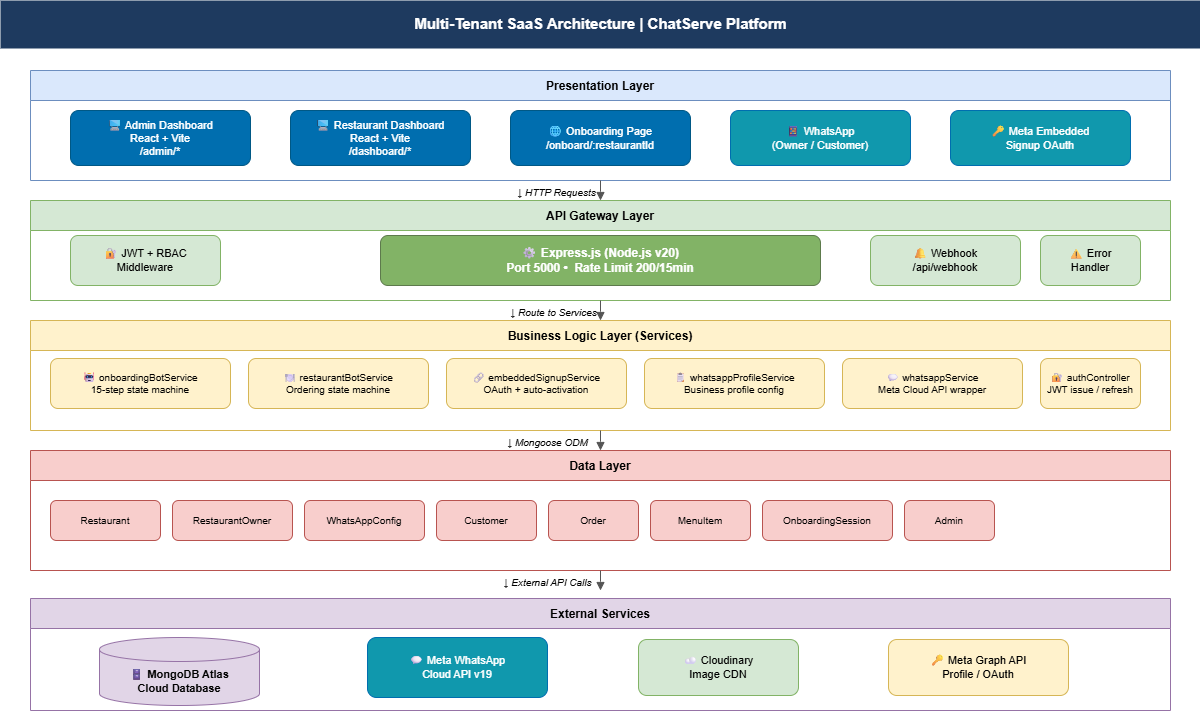
\includegraphics[width=0.99\textwidth]{Diagrams/system_architecture.png}
\caption{Overall System Architecture of ChatServe}
\label{fig:system_architecture}
\end{figure}

Above we present an architecture diagram which shows off the interaction between the frontend dashboards, Express.js backend, MongoDB database, and the Meta WhatsApp Cloud API. We see the message flow in through webhooks and are also show how various business tenants use the same back end infrastructure but at the same time have fully isolated data through the use of tenant scoped queries.


In a multi-tenant model we use a \textbf{shared database, shared schema} approach. Each data record for a business has a \texttt{business} ObjectId which is true for all of them and we at the API query level scope to the authenticated tenant's ID which is at the middleware layer. Thus we achieve full logical isolation between tenants at the same time we keep the infrastructure simple and cost effective.

\section{System Flow}

\subsection*{Business Onboarding Flow}

The business owner kicks off the onboarding process by sending the first message on WhatsApp. We have done away with the traditional form in favor of a guided chat which steps the user through the process. The bot puts out a series of questions which include the owner's name, business name, contact info, address, description, operating hours, business category, products or services and logo. As each response is received in real time they are stored which in turn improves accuracy and completeness.

\begin{figure}[H]
\centering
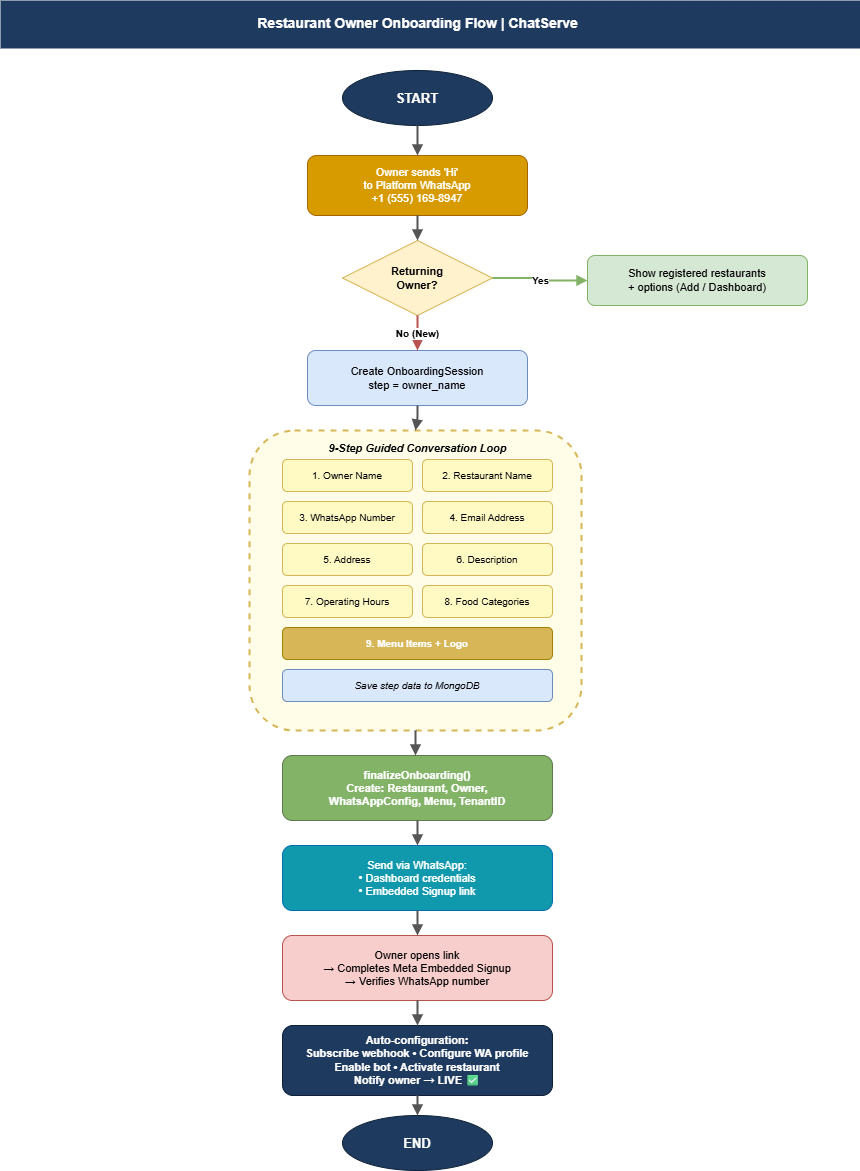
\includegraphics[width=0.85\textwidth]{Diagrams/Onboarding Flow.png}
\caption{Business Onboarding Flow via WhatsApp}
\label{fig:onboarding_flow}
\end{figure}

Once we have all the details we put together the required database records and we provide the owner a unique Embedded Signup link along to which they can access their dashboard also we give them login info. We have a very structured process in which each step is checked off before we move on to the next which in turn guarantees consistent and reliable data collection through out the onboarding.


\subsection*{Onboarding Sequence Diagram}
The diagram below shows in more detail the interaction between the business owner, the ChatServe backend, the MongoDB database, and the Meta WhatsApp Cloud API during the onboarding process. 

\begin{figure}[H]
\centering
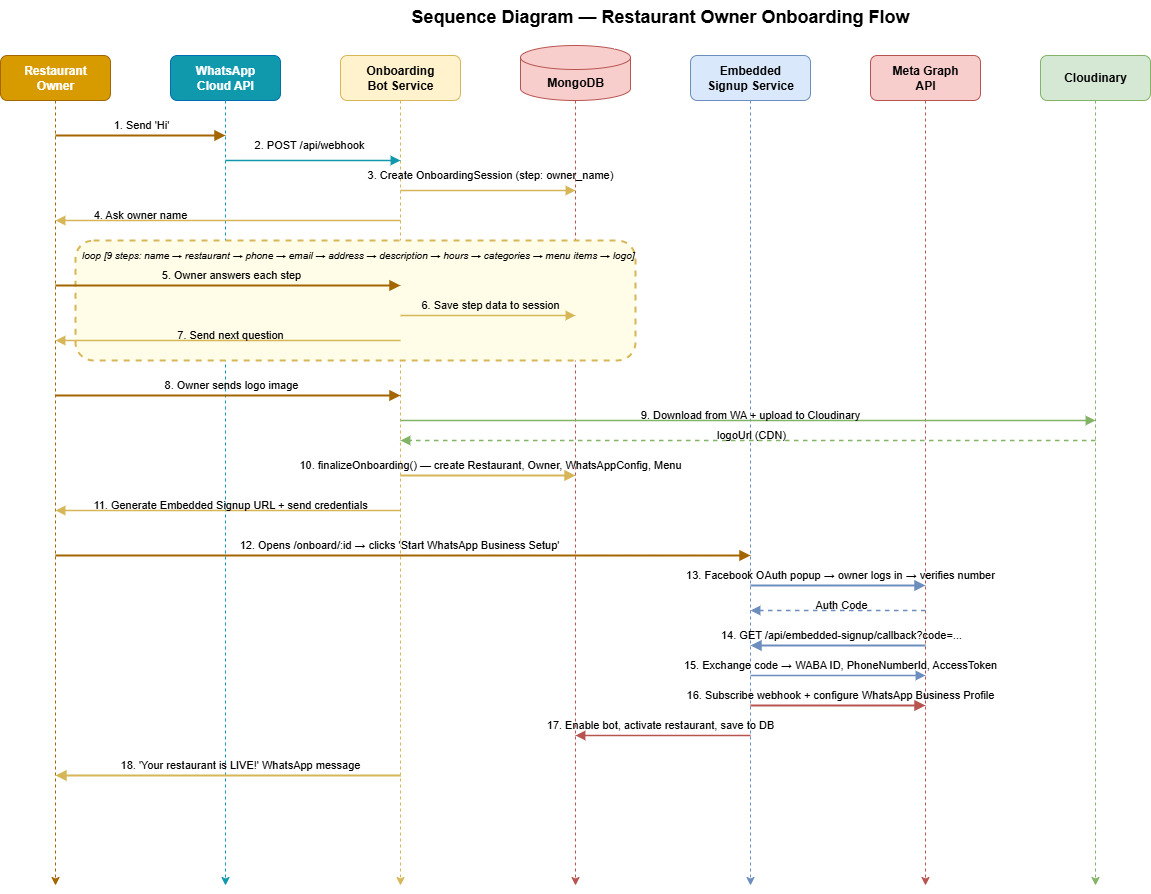
\includegraphics[width=0.99\textwidth]{Diagrams/Sequence_diagram - restauretn_Onboarding.png}
\caption{Sequence Diagram for Business Onboarding}
\label{fig:seq_onboarding}
\end{figure}

In the sequence diagram we see that each of owner's messages trigger a webhook POST to the backend. The backend which at this point is reading the present session state from MongoDB, determining the next move, out via the Meta API returns a response and also updates the session. This is a stateless request response cycle which plays out till we complete the tenth of the on boarding steps at which point the backend in question creates all tenant records and we dispatch the Embedded Signup link.

\subsection*{Customer Ordering Flow}

When a customer messages the business's WhatsApp number the webhook handler out of which the phone number is identified, we then go on to retrieve the customer and their session at the business, and the message is sent to the business bot. The bot in turn displays a very interactive main menu to the customer, allows them to look through categories and products or services, add what they like to a persistent cart, take them through a 3 step check out (address, confirm, pay) and at the end gives out an order confirmation message with a unique order ID. Also if the business owner updates any order status that change is immediately sent out to the customer via a WhatsApp message.

\subsection*{Customer Order Sequence Diagram}

\begin{figure}[H]
\centering
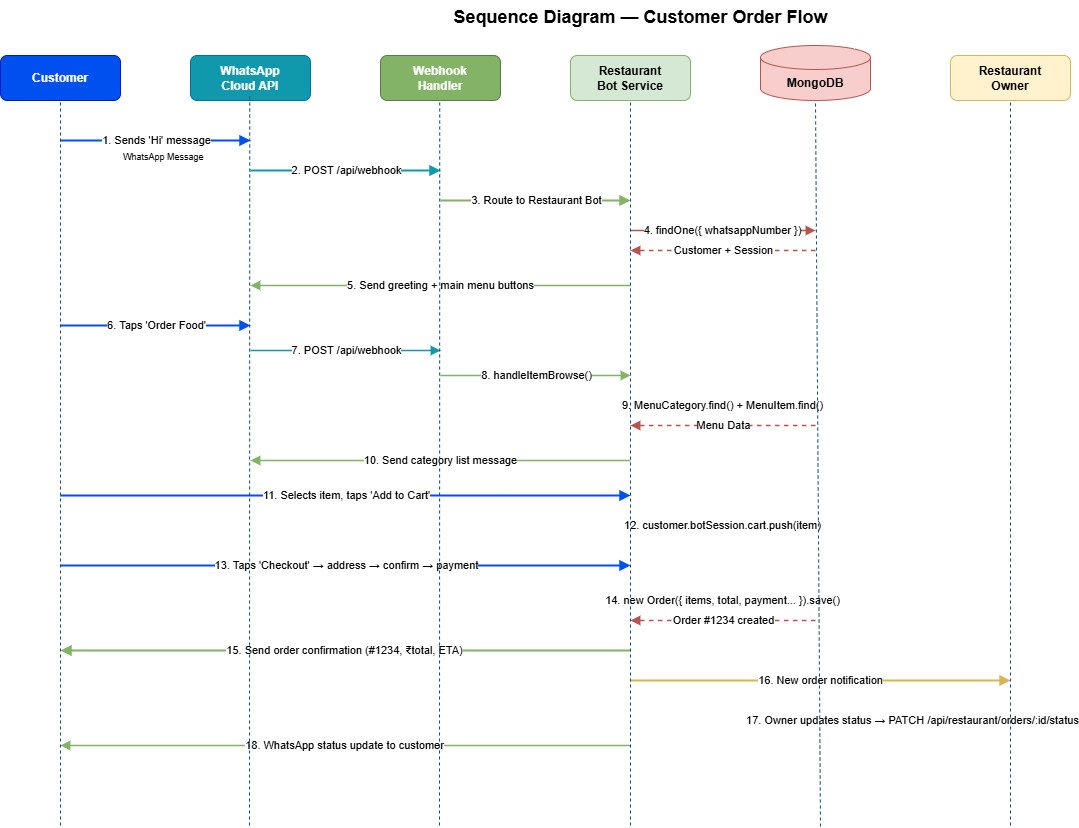
\includegraphics[width=0.90\textwidth]{Diagrams/Sequence_Diagram- cutomer_Order Flow.png}
\caption{Sequence Diagram for Customer Order Flow}
\label{fig:seq_ordering}
\end{figure}

The customer flow Sequence diagram which details the full message exchange from the time of the customer's first interaction through to the order confirmation. We see how the webhook routes messages to the proper business's bot, how we maintain the cart state between multiple exchanges, and how the final order is put into the database and reported back to the customer via WhatsApp.

\section{Database Design}

ChatServe uses MongoDB for it's primary data storage. We have designed the schema around the Business document which is our main focus. Also listed below are the key collections and their relationships.

\begin{figure}[H]
\centering
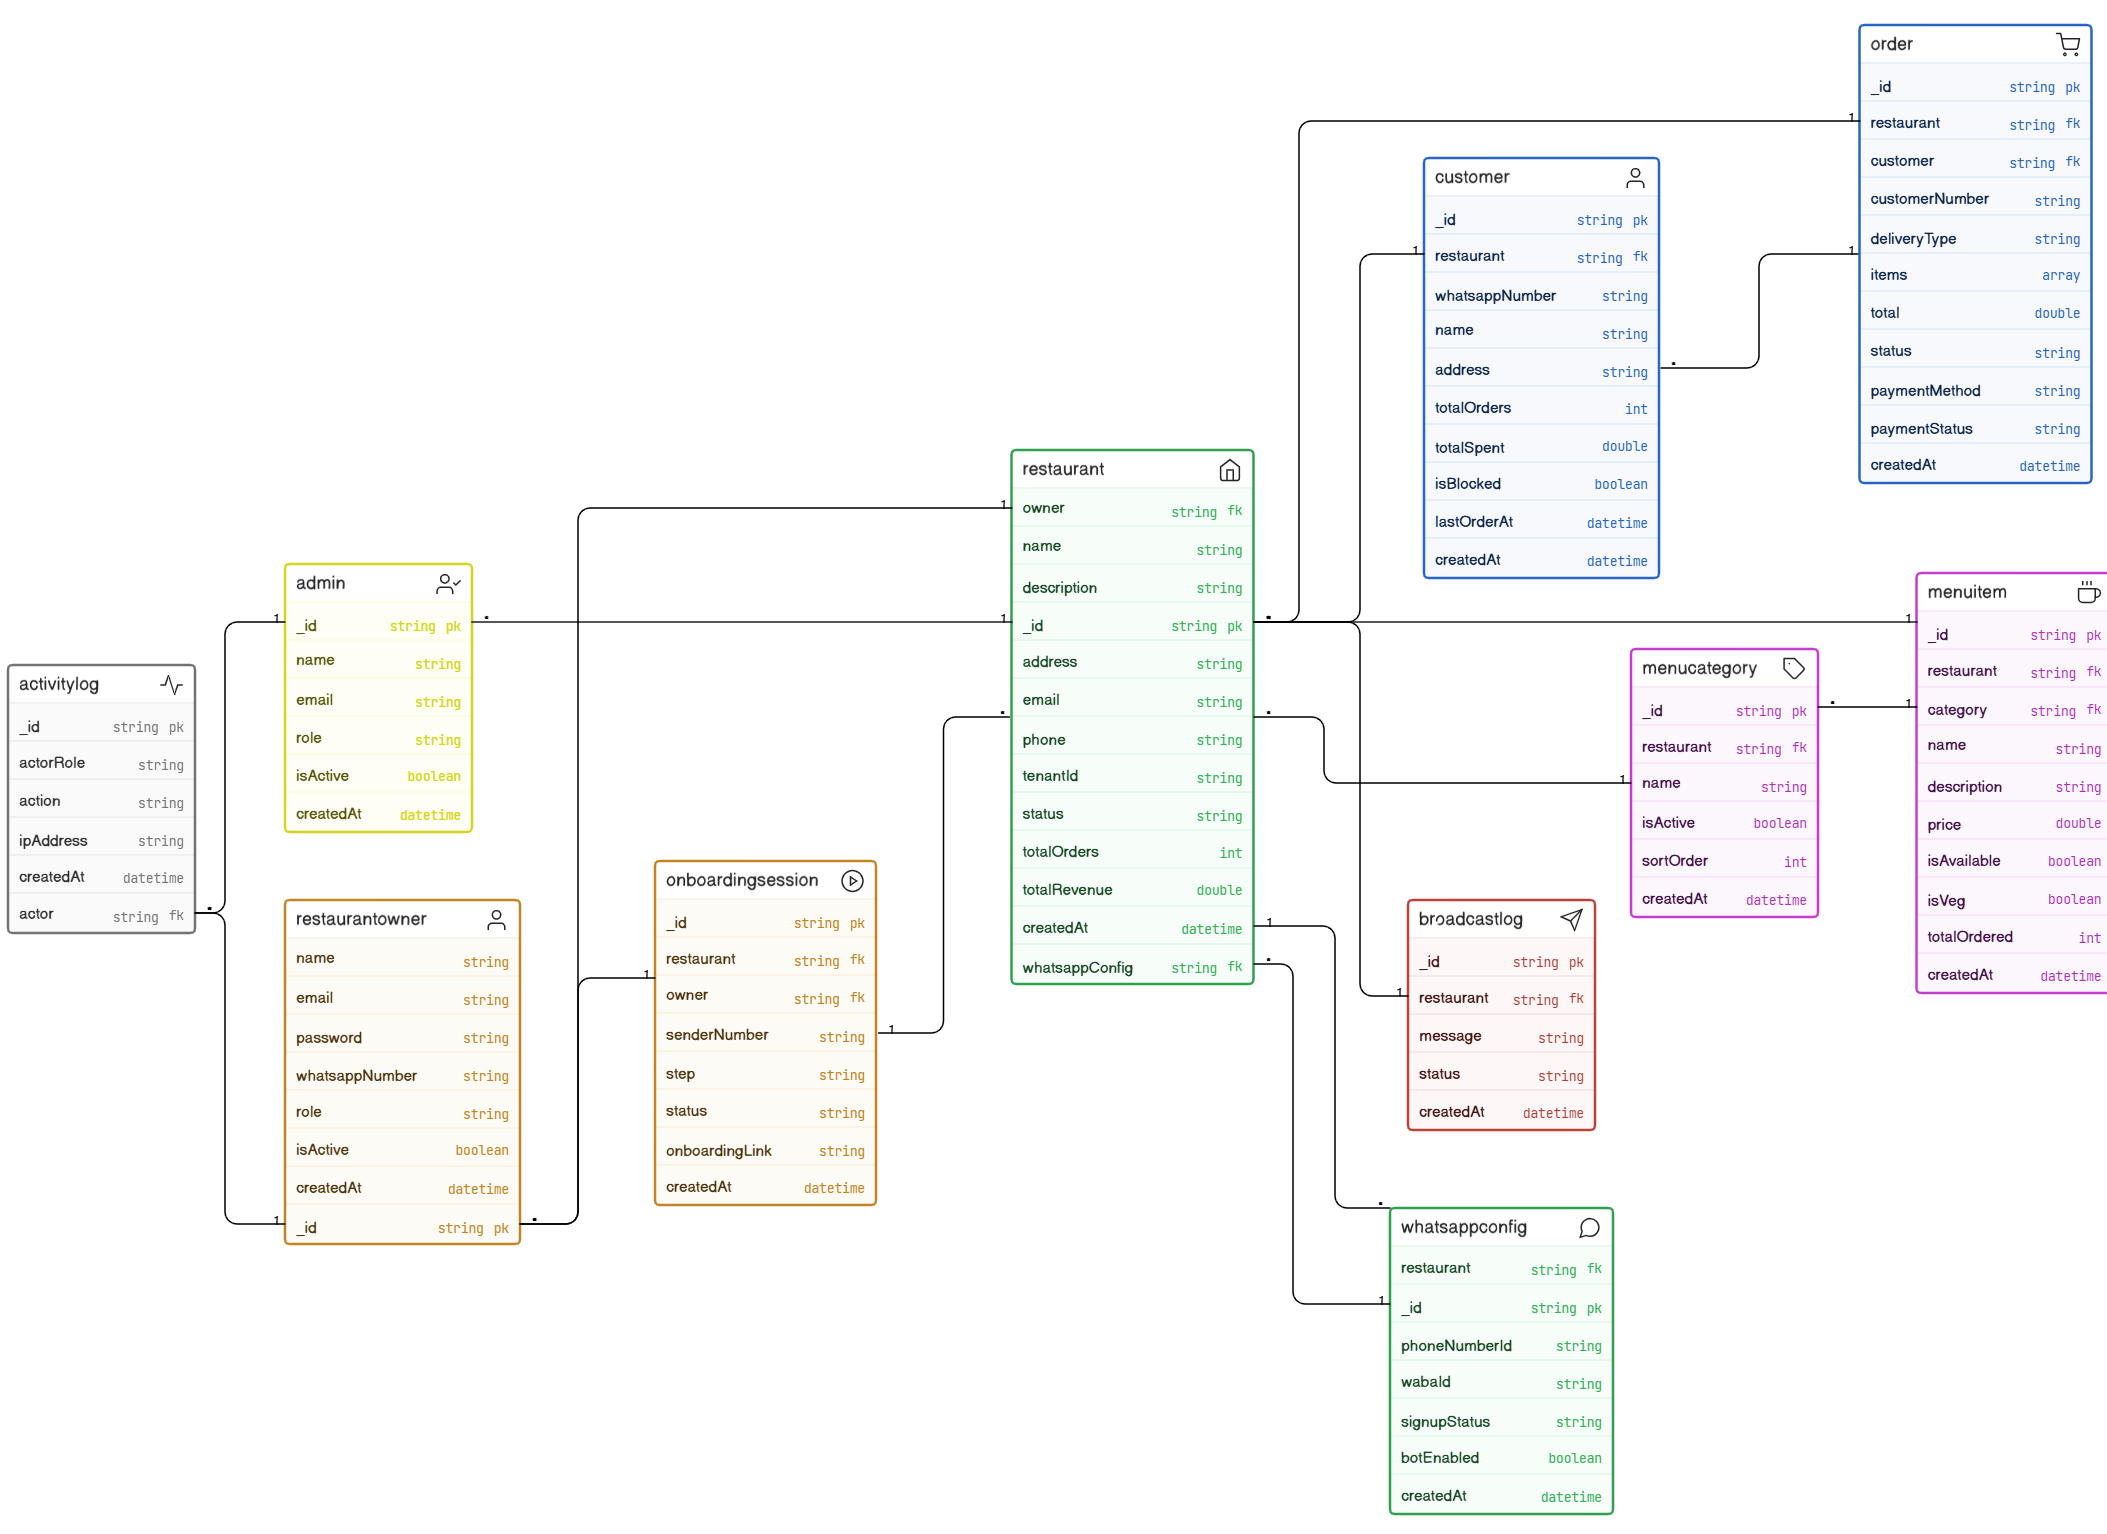
\includegraphics[width=0.99\textwidth]{Diagrams/er_diagram.png}
\caption{Entity-Relationship Diagram for the ChatServe Database}
\label{fig:er_diagram}
\end{figure}

In the diagram we present how each core collection interrelate which in turn serves as the root tenant for all other records. We have the WhatsAppConfig which puts in place Meta API credentials per business, Customer documents which we use for session and cart state and Order documents which cover the full order lifecycle. Also we use MongoDB ObjectIds for all foreign key references and have the businessId field indexed in each collection which in turn supports efficient tenant scoped queries.


\begin{itemize}

    \item \textbf{Business}: Core element document which includes business details, status, and which also puts forth all related collections.
    
    \item \textbf{BusinessOwner}: Auth info and contact details for the dashboard user.
    
    \item \textbf{WhatsAppConfig}: WABA ID, Phone Number ID, access token, webhook subscription status, and bot enable flag.
    
    \item \textbf{Customer}: Per each unique WhatsApp number per business we have the bot session state and cart.
    
    \item \textbf{CatalogItem}: Product/service catalog with pricing, category, availability and Cloudinary image URL.
    
    \item \textbf{Order}: Full order record including items, total, payment method, status and also a status history array.
    
    \item \textbf{OnboardingSession}: Goes over the registration progress of business owners which are in the process of on boarding.
    
    \item \textbf{Admin}: Platform admin credentials.

\end{itemize}

\begin{table}[H]
\centering
\caption{Core Collections and Key Fields}
\renewcommand{\arraystretch}{1.3}
\begin{tabularx}{\textwidth}{|l|X|}
\hline
\textbf{Collection} & \textbf{Key Fields} \\
\hline
businesses & name, status, tenantId, owner \\
\hline
whatsappconfigs & wabaId, phoneNumberId, botEnabled \\
\hline
customers & whatsappNumber, botSession, cart \\
\hline
orders & orderNumber, items, total, status \\
\hline
catalogitems & name, price, category, isAvailable \\
\hline
onboardingsessions & step, data, senderNumber \\
\hline
\end{tabularx}
\end{table}

\section{Implementation Details}

\subsection{Backend Implementation}

The backend is developed with Node.js and Express.js which we have structured into a modular architecture. This we did in order to put business logic at the charge of dedicated service layers from the route hander's perspective. In terms of the results we see enhanced maintainability and a better model of code organization.

\begin{lstlisting}[caption=Backend Directory Structure]
backend/
├── .env
├── .gitignore
├── config/
│   ├── cloudinary.js
│   ├── db.js
│   └── redis.js
├── controllers/
│   └── authController.js
├── middleware/
│   ├── auth.js
│   ├── errorHandler.js
│   └── upload.js
├── models/
│   ├── Admin.js
│   ├── Customer.js
│   ├── Logs.js
│   ├── Menu.js
│   ├── OnboardingSession.js
│   ├── Order.js
│   ├── Restaurant.js
│   ├── RestaurantOwner.js
│   └── WhatsAppConfig.js
├── package-lock.json
├── package.json
├── routes/
│   ├── admin.js
│   ├── analytics.js
│   ├── auth.js
│   ├── embeddedSignup.js
│   ├── menu.js
│   ├── onboarding.js
│   ├── order.js
│   ├── restaurant.js
│   ├── upload.js
│   └── webhook.js
├── server.js
├── services/
│   ├── emailService.js
│   ├── embeddedSignupService.js
│   ├── notificationService.js
│   ├── onboardingBotService.js
│   ├── restaurantBot/
│   │   ├── commands.js
│   │   ├── context.js
│   │   ├── index.js
│   │   ├── steps/
│   │   │   ├── cart.js
│   │   │   ├── checkout.js
│   │   │   ├── greeting.js
│   │   │   ├── help.js
│   │   │   ├── mainMenu.js
│   │   │   ├── menuBrowse.js
│   │   │   └── orders.js
│   │   └── utils/
│   │       └── messenger.js
│   ├── restaurantBotService.js
│   ├── whatsappProfileService.js
│   └── whatsappService.js
├── templates/
│   └── emails/
│       └── passwordReset.html
└── utils/
    ├── helpers.js
    ├── jwt.js
    ├── logger.js
    ├── phoneUtils.js
    └── seed.js

\end{lstlisting}

The chatbot modules present an approach which is state based, in that each user interaction is processed according to the current session state which is in MongoDB. Each incoming message sets off a state transition which in turn enables structured conversational flows like onboarding and order placement. We receive all WhatsApp messages via a webhook endpoint. The backend processes each request and routes it based on the associated phone number. At the platform level we have the onboarding bot which handles that traffic, at the business specific level we have separate ordering bots which do the processing, thus we achieve accurate handling in a multi tenant system.


\subsection{Frontend Implementation}

The frontend of our application is a React 18 Single Page Application which we built using Vite and we styled it with Tailwind CSS. We use TanStack Query for efficient server state management and caching.

\begin{lstlisting}[caption=Frontend Directory Structure, captionpos=b]
frontend/
├── .gitignore
├── index.html
├── package-lock.json
├── package.json
├── postcss.config.js
├── src/
│   ├── App.jsx
│   ├── components/
│   │   ├── PasswordResetModal.jsx
│   │   └── common/
│   │       └── StatCard.jsx
│   ├── context/
│   │   └── AuthContext.jsx
│   ├── index.css
│   ├── layouts/
│   │   ├── AdminLayout.jsx
│   │   └── RestaurantLayout.jsx
│   ├── main.jsx
│   ├── pages/
│   │   ├── admin/
│   │   │   ├── Broadcast.jsx
│   │   │   ├── Dashboard.jsx
│   │   │   ├── Onboarding.jsx
│   │   │   ├── RestaurantDetail.jsx
│   │   │   └── Restaurants.jsx
│   │   ├── auth/
│   │   │   ├── LoginPage.jsx
│   │   │   ├── OnboardError.jsx
│   │   │   ├── OnboardPage.jsx
│   │   │   └── OnboardSuccess.jsx
│   │   └── restaurant/
│   │       ├── Broadcast.jsx
│   │       ├── Customers.jsx
│   │       ├── Dashboard.jsx
│   │       ├── Menu.jsx
│   │       ├── Orders.jsx
│   │       ├── Profile.jsx
│   │       └── WhatsApp.jsx
│   └── services/
│       └── api.js
├── tailwind.config.js
└── vite.config.js

\end{lstlisting}

The application has role based designs for Admin and Business Owner users. We use JWT tokens for authentication. Access tokens are of 15 minute duration and issue refresh tokens which are valid for 7 days. We include auth headers in API requests and we have put in place a silent token refresh which takes care of expired sessions thus providing a smooth user experience.


\section{System Features and Functionalities}

The presented system reports an extensive set of features which we put forward for business onboarding, order and booking management, and customer interaction via WhatsApp.

\begin{itemize}

\item \textbf{Platform Onboarding Bot:}
A chatbot that walks business owners through a series of steps in the registration process on WhatsApp. It supports text input, image upload, session management, and the auto creation of required database entries. At the end we provide login info to the owner.

\item \textbf{Meta Embedded Signup Integration:}
Enables the business to connect with WhatsApp Business API which is a service of Meta via our OAuth based Embedded Signup flow. We auto fill in the required info and take care of backend config which includes setting up webhooks and activating the bot.

\item \textbf{Automatic WhatsApp Business Profile Configuration:}
Automatically maintains the business's WhatsApp Business profile via Meta Graph API. We sync business name, description, category, and contact info with the platform data.

\item \textbf{Business Ordering Bot:}
An interactive chatbot that which customers use to go through product or service categories, see available offerings, put things in their cart, and place orders. We have a structured checkout process and also we which remember customer context for return users.

\item \textbf{Business Owner Dashboard:}
A web based platform which includes key functions of order management, product/service catalog update, customer tracking, and basic analytics which in turn includes order trends, and revenue reports.

\item \textbf{Super Admin Dashboard:}
Centralized to all aspects of the platform which includes business management, onboarding, monitoring, system configuration, and broadcast communication with business owners.

\end{itemize}


\section{Results}

Screenshots illustrating the complete functionality of the created platform are provided below for each of the three user types.

\begin{figure}[H]
\centering
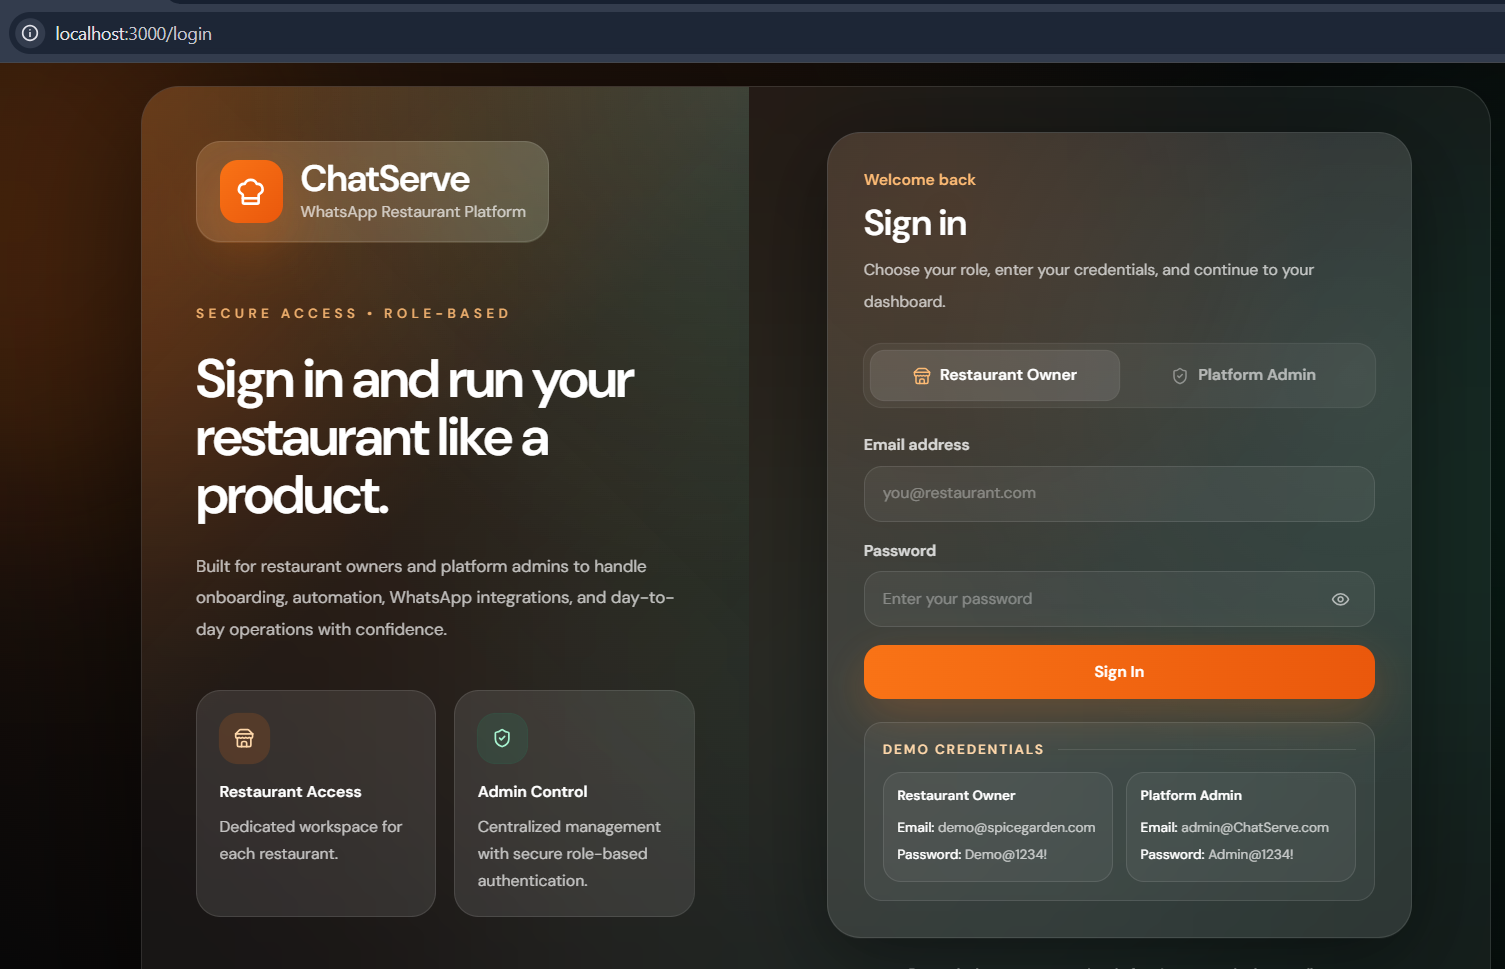
\includegraphics[width=0.80\textwidth]{Diagrams/loginpage.png}
\caption{Login Page for Super Admin and Business Owner}
\label{fig:login}
\end{figure}

The login page provides role-based authentication that directs admins to the Super Admin dashboard and business owners to their personal account page. The session is protected by the JWT mechanism, with access tokens expiring after 15 minutes and refreshing after 7 days.

\subsection{Business Registration via WhatsApp}
Below you can see the actual WhatsApp conversation between a business owner and the bot guiding the latter in the registration process. The bot asks all the necessary questions, and the owner just needs to answer them.

\begin{figure}[H]
\centering
\begin{minipage}{0.48\textwidth}
    \centering
    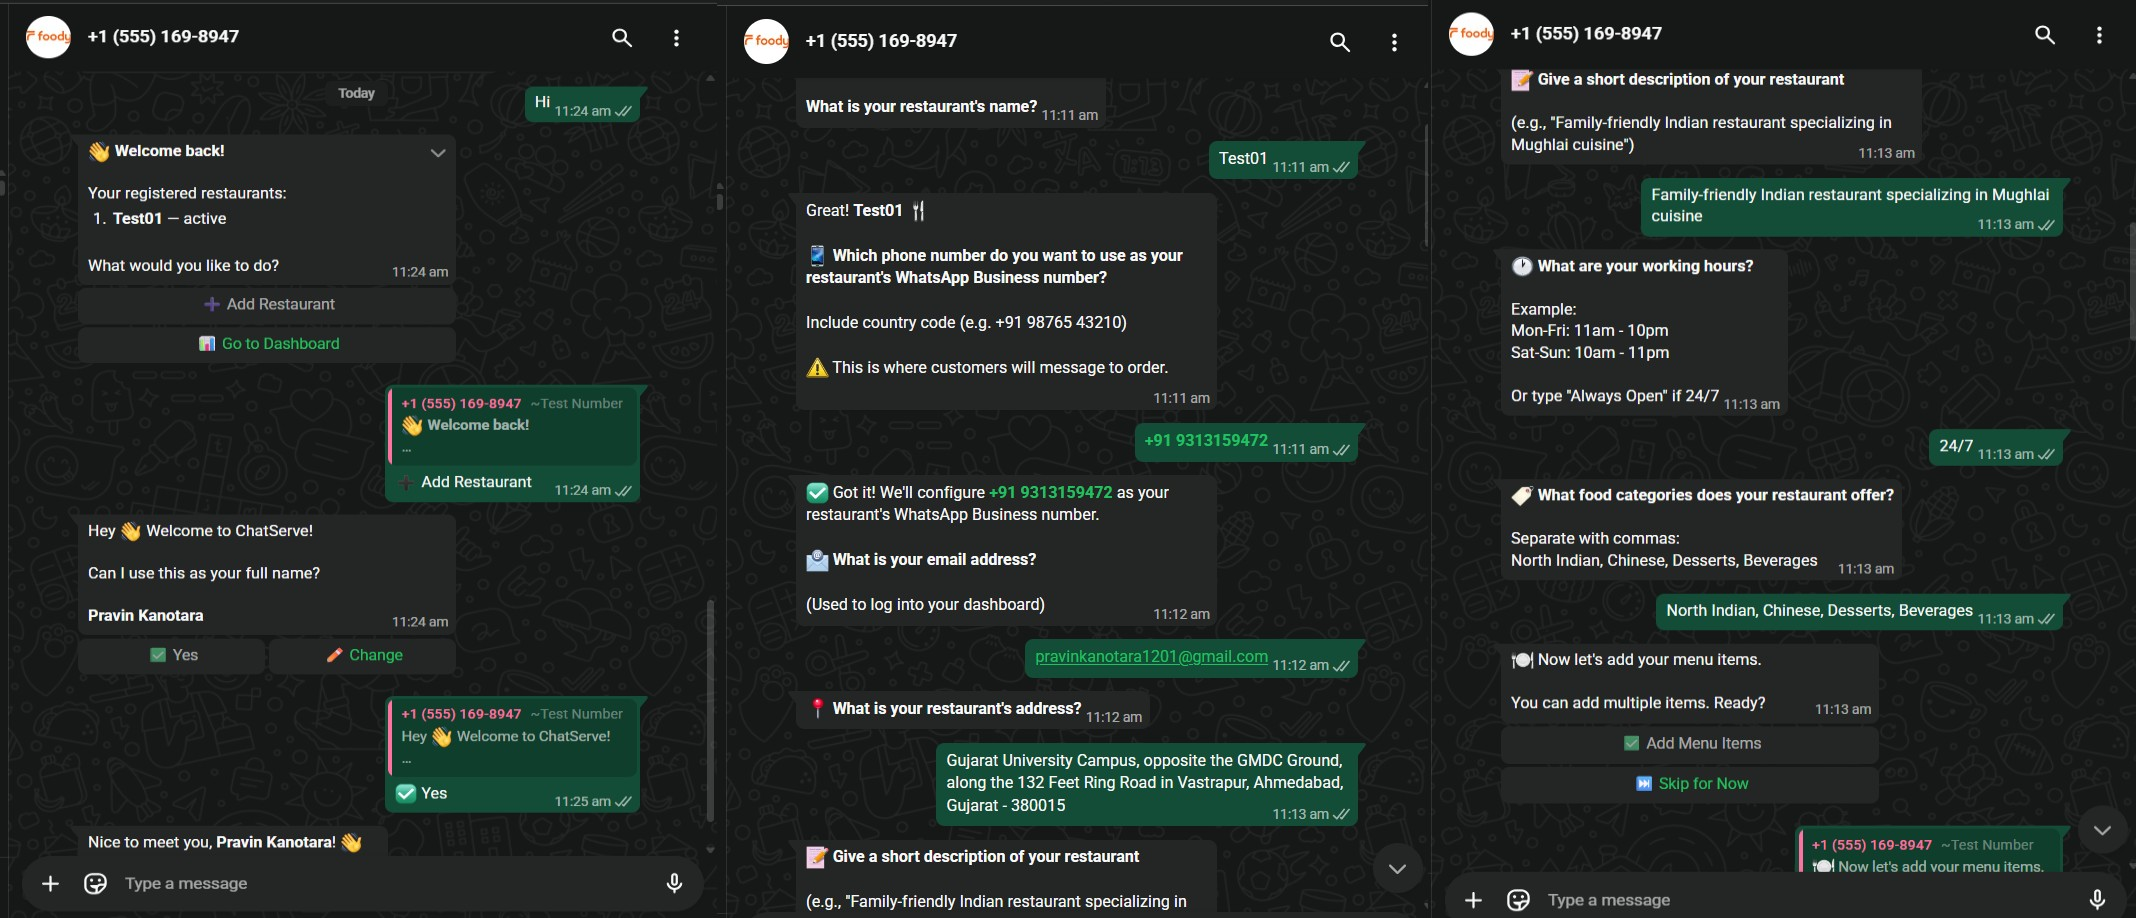
\includegraphics[width=\linewidth]{Diagrams/restaurant_reg1_3.jpg}
    \caption*{(a) Steps 1-3: Owner's name, business name, WhatsApp number}
\end{minipage}
\hfill
\begin{minipage}{0.48\textwidth}
    \centering
    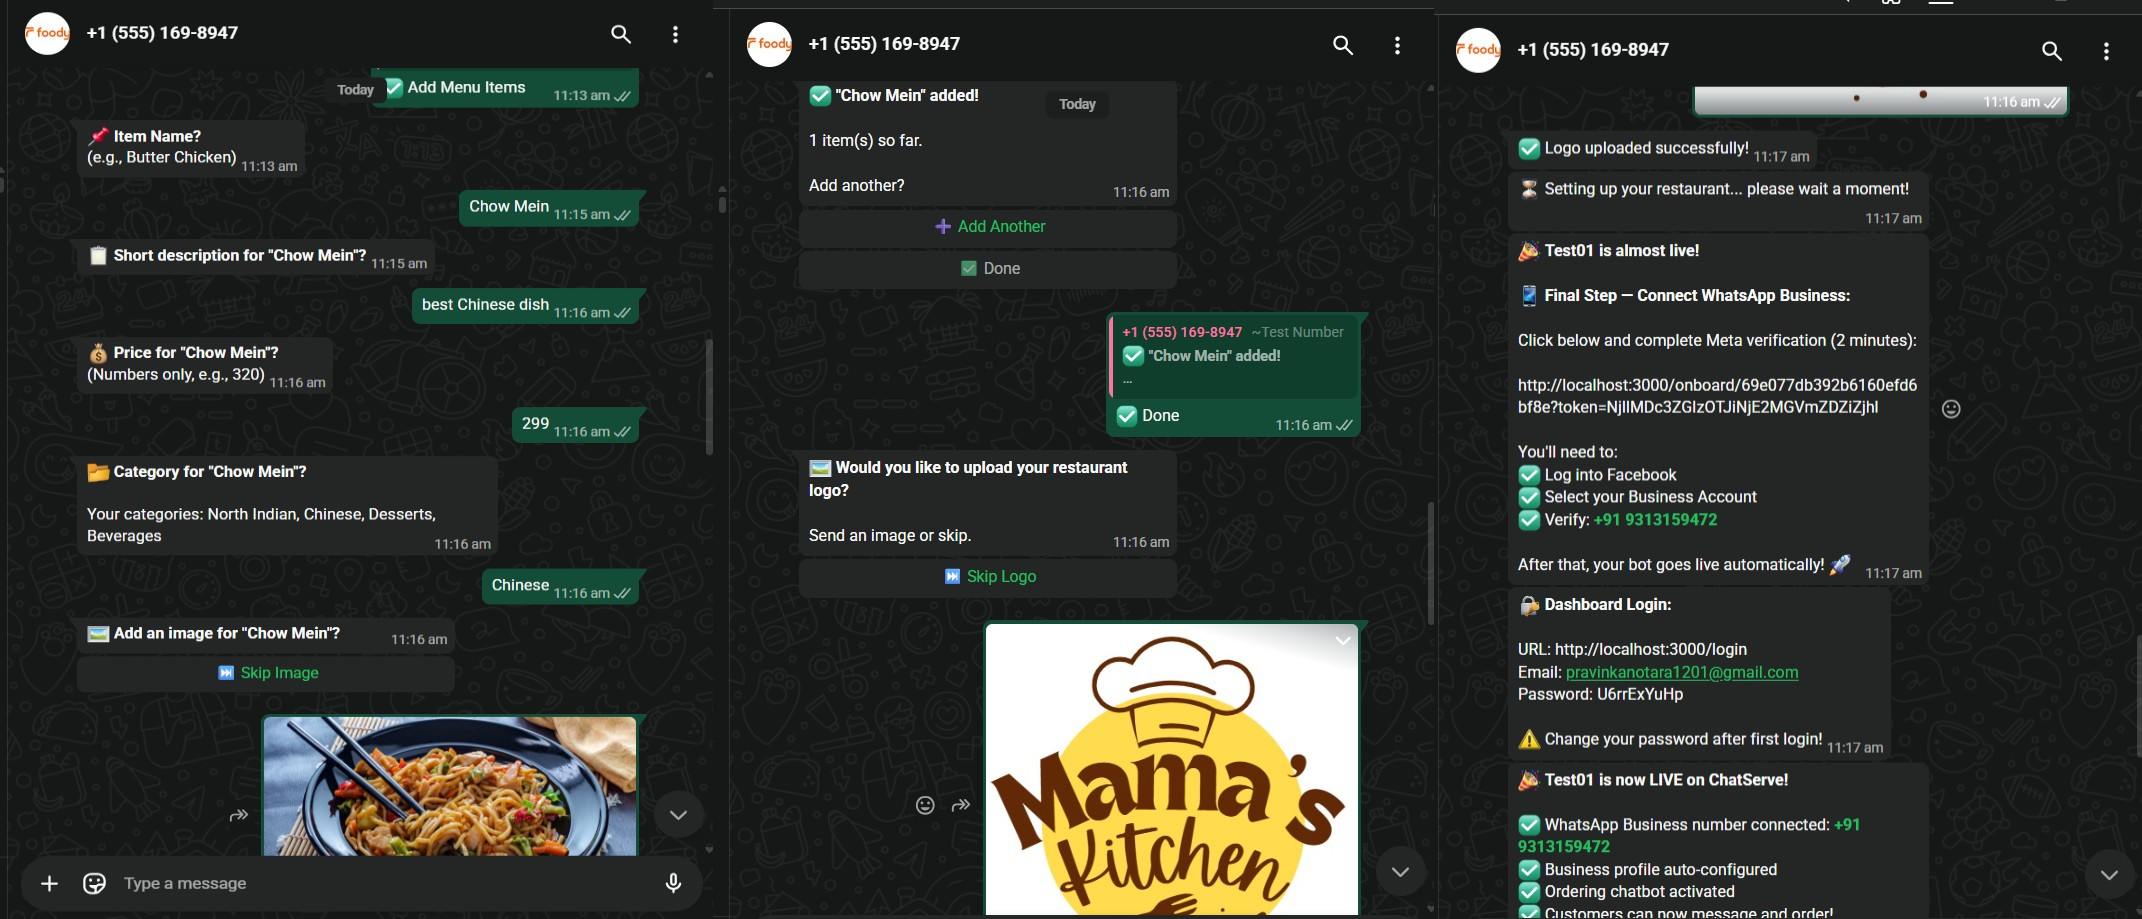
\includegraphics[width=\linewidth]{Diagrams/restaurant_reg_4_6.jpg}
    \caption*{(b) Steps 4-6: Email address, business address, description}
\end{minipage}
\caption{Actual WhatsApp Onboarding Process for Business Owners}
\label{fig:wa_registration}
\end{figure}

From the above, it becomes clear that the onboarding process is fully conversational and is carried out completely inside WhatsApp messenger. Furthermore, every question posed by the bot to the business owner gets validated, and the bot will repeat itself in case of an invalid response.

\subsection{Admin Dashboard and Controls}

\begin{figure}[H]
\centering
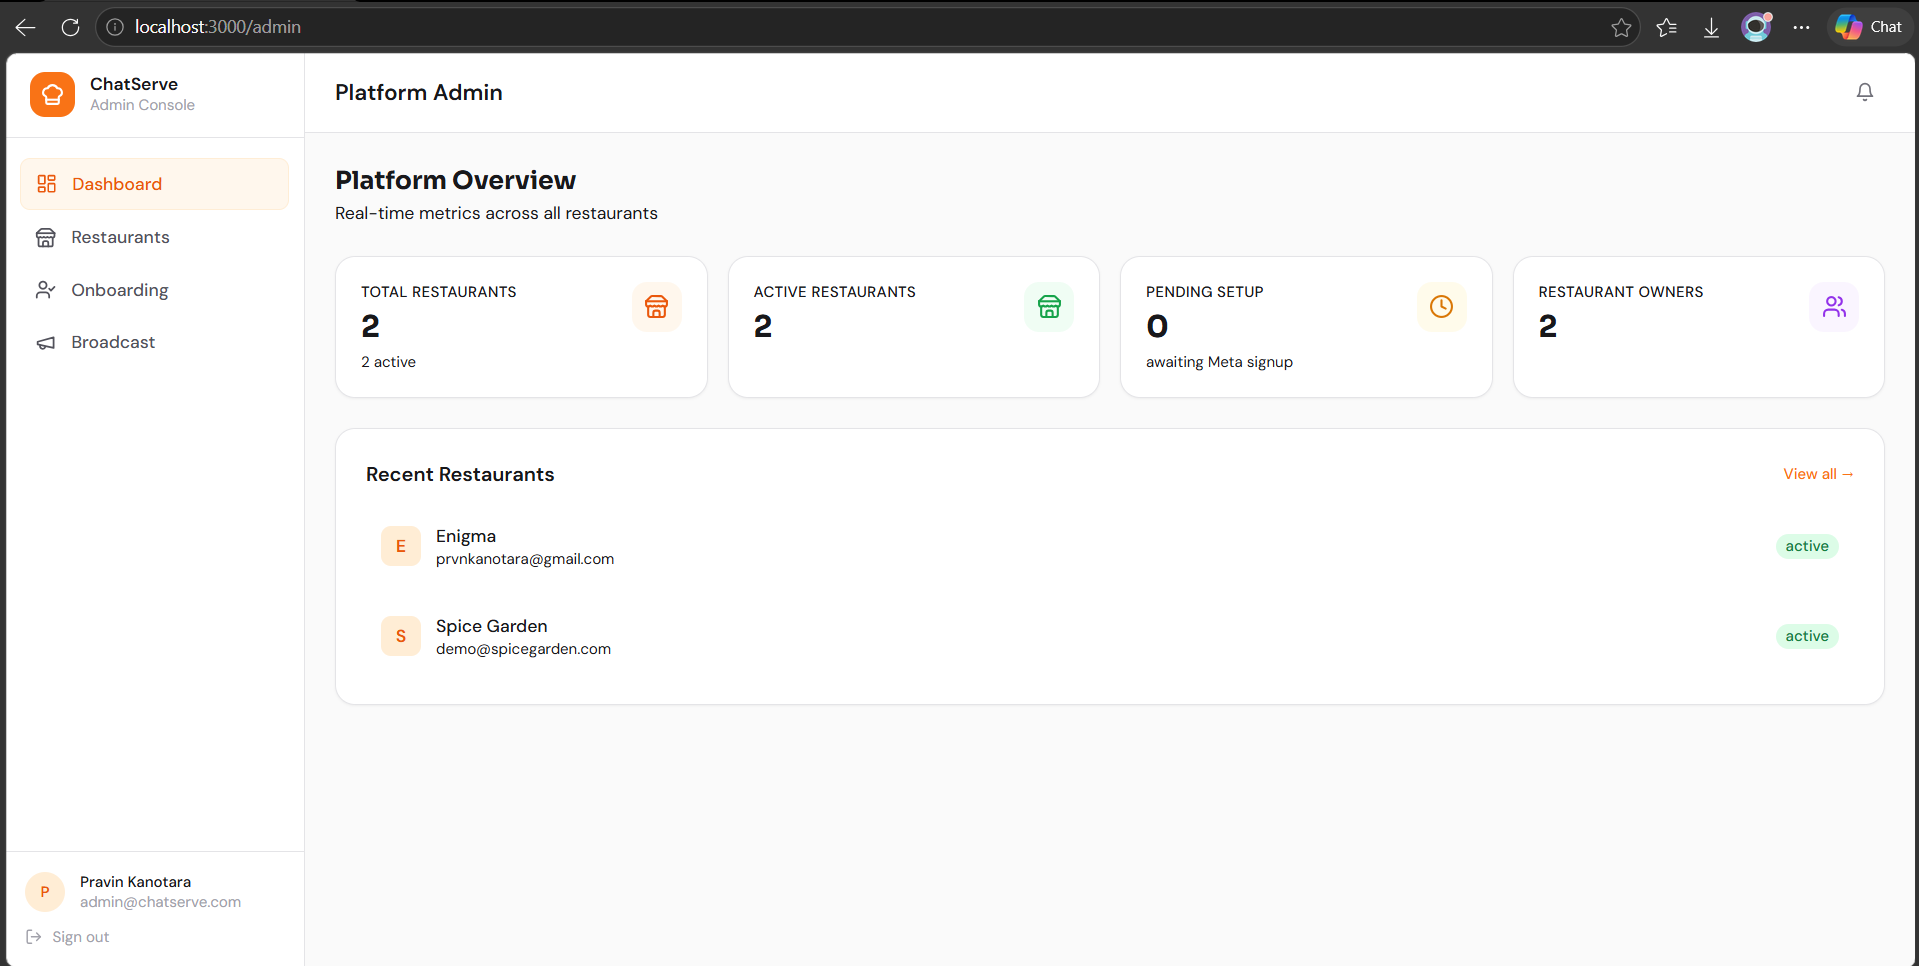
\includegraphics[width=0.95\textwidth]{Diagrams/admin_dashboard .png}
\caption{Admin Dashboard: Platform KPIs Overview and Businesses Listing}
\label{fig:admin_dashboard}
\end{figure}

The administrator sees a general overview of all activities occurring within the platform. It includes KPIs like the total number of registered businesses, active bots, order count and other metrics. Furthermore, it is possible to open a detailed view for each individual business to either activate/deactivate it or to configure its WhatsApp integration.

\begin{figure}[H]
\centering
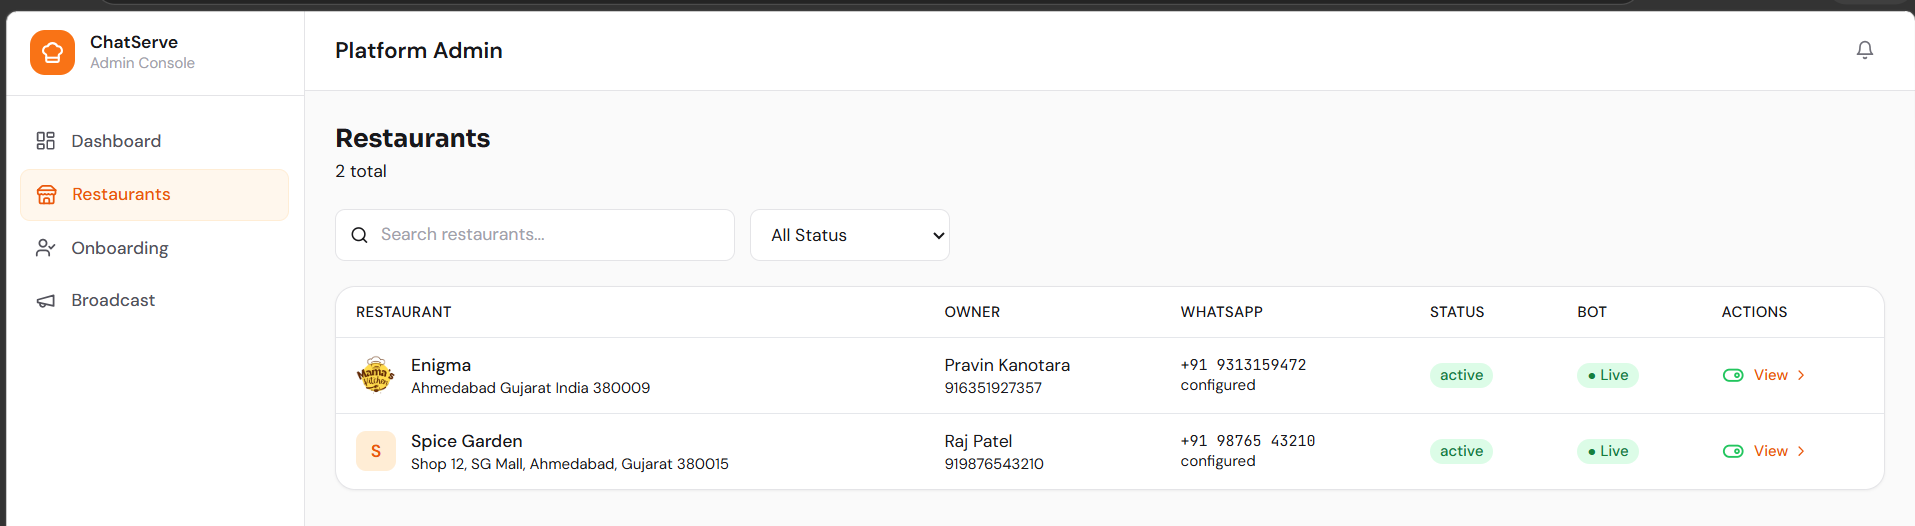
\includegraphics[width=0.95\textwidth]{Diagrams/admin_restaurents.png}
\caption{Listing of Registered Businesses on Admin Interface}
\label{fig:admin_restaurants}
\end{figure}

Here the business is presented in the list along with its current activation status (pending, active or suspended). It also has an icon that allows opening a page with detailed settings for that business or manually activating/deactivating its WhatsApp configuration.

\begin{figure}[H]
\centering
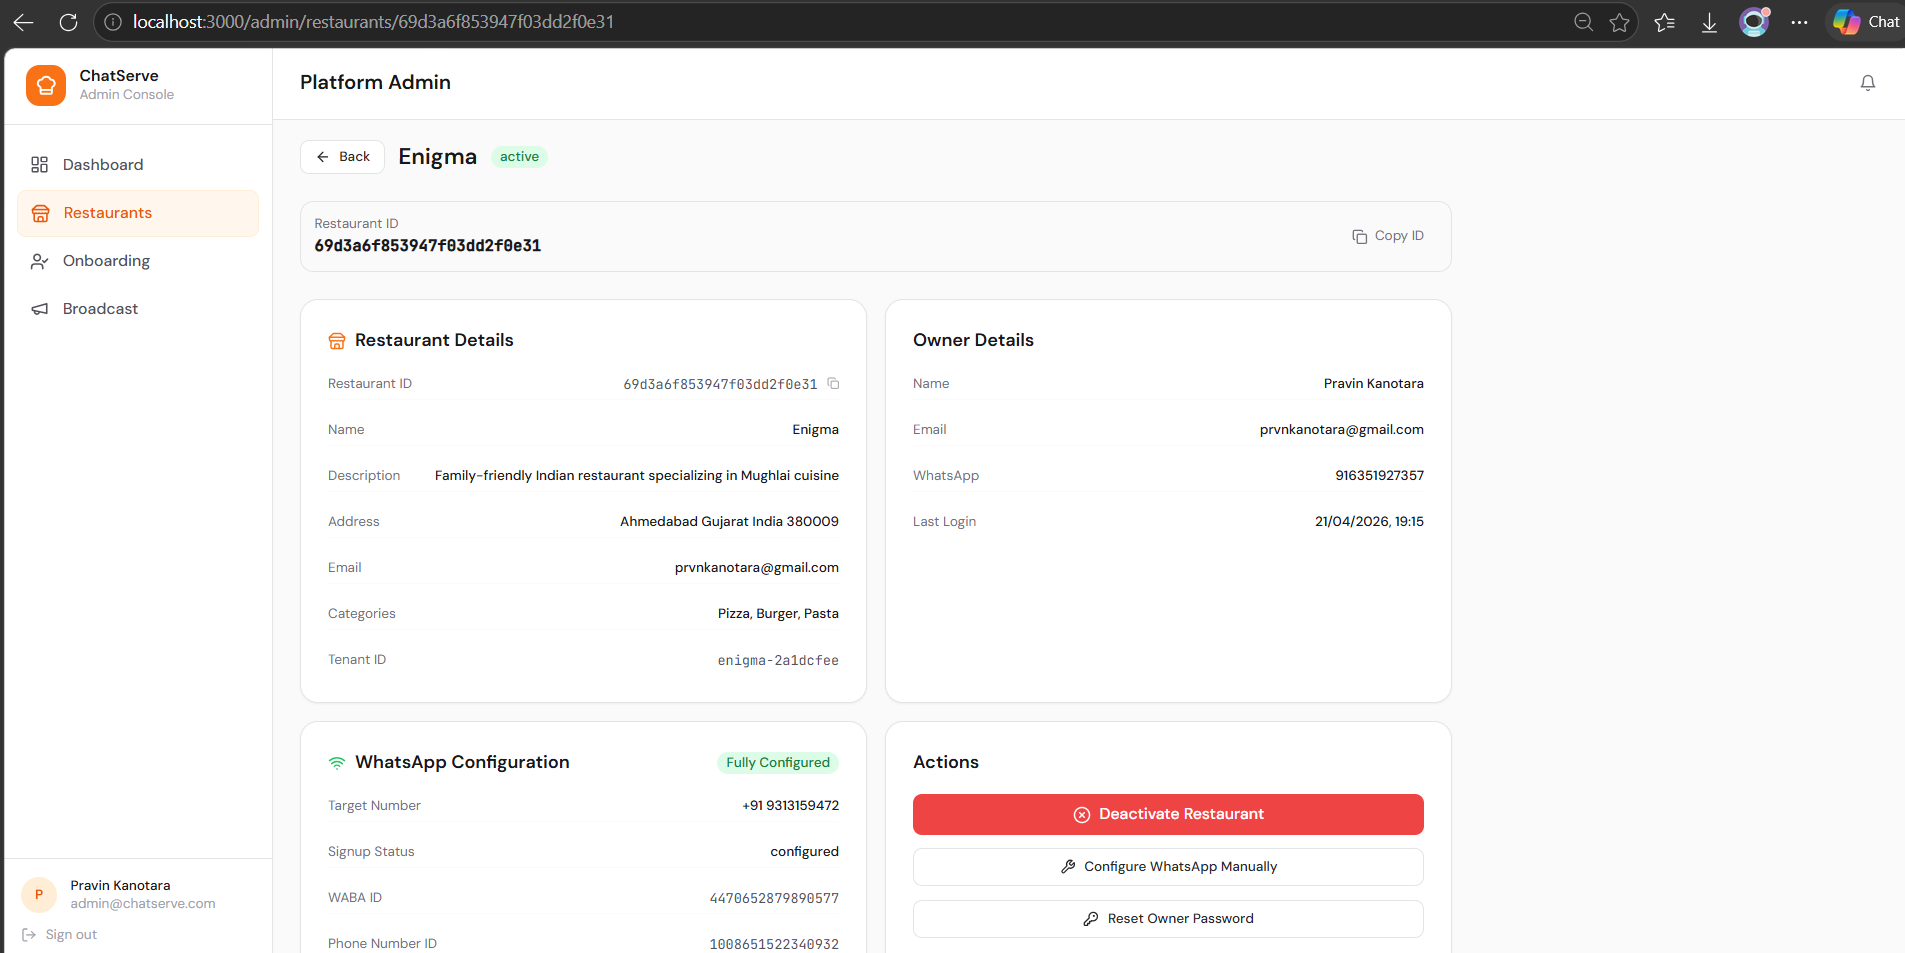
\includegraphics[width=0.95\textwidth]{Diagrams/admin_restaurent_details.png}
\caption{Detailed Information about a Business}
\label{fig:admin_restaurant_detail}
\end{figure}

As seen from above, the business detail view provides an administrator with important information such as WhatsApp Business Account ID, Phone Number ID, webhook endpoint validation status, and status of its bot. In addition, the administrator can use the ``manual setup'' block to populate WhatsApp integration information manually.

\begin{figure}[H]
\centering
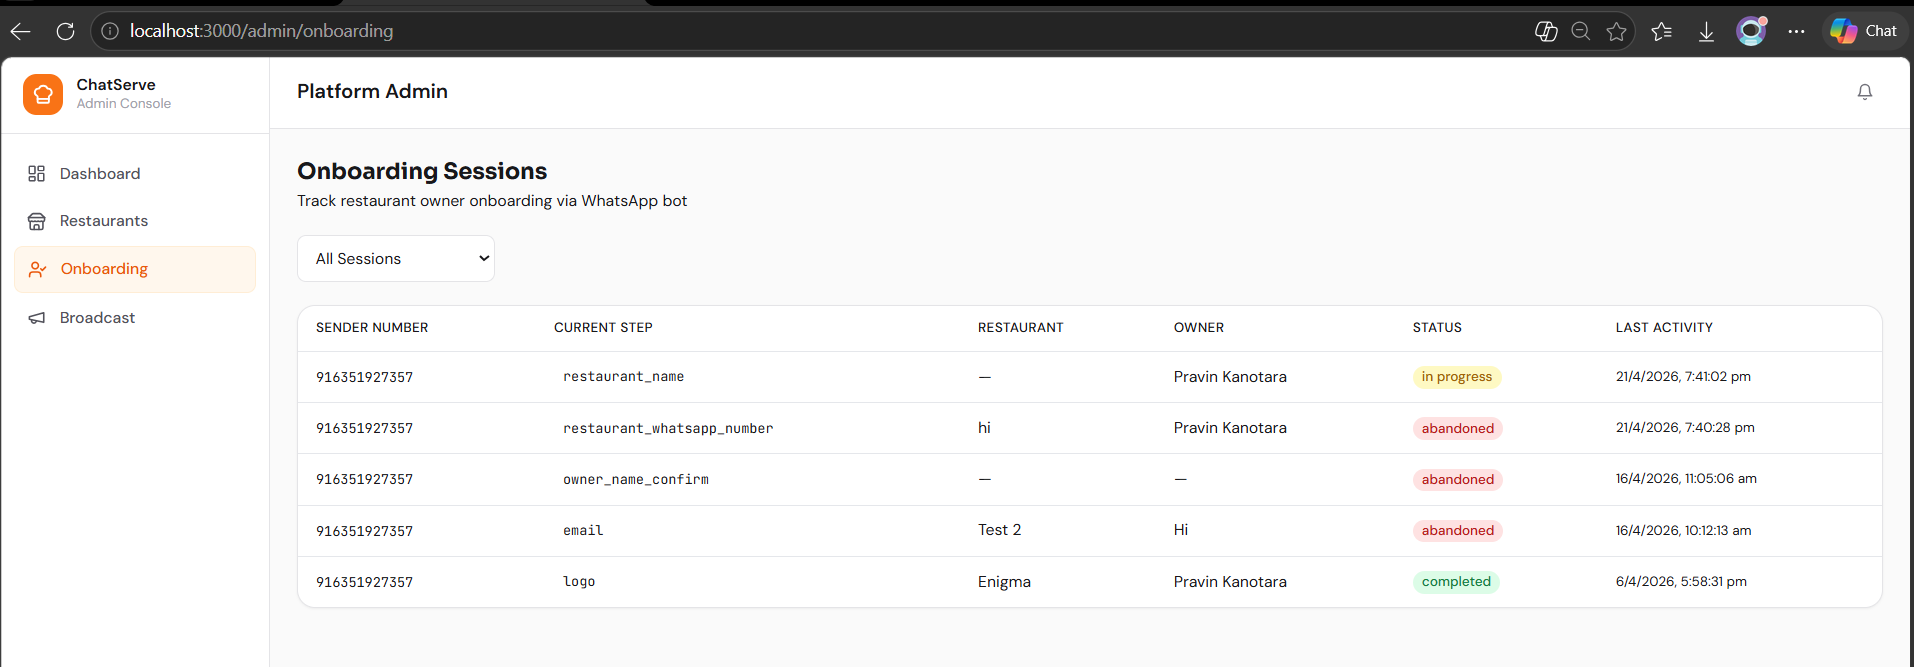
\includegraphics[width=0.95\textwidth]{Diagrams/admin_onboarding.png}
\caption{Dashboard: Ongoing Onboarding Sessions Monitor}
\label{fig:admin_onboarding}
\end{figure}

Here the platform administrator has live monitoring of all ongoing onboarding processes. For each ongoing session the administrator knows the WhatsApp number of the sender, the question number they are at now and the time when the session started.

\begin{figure}[H]
\centering
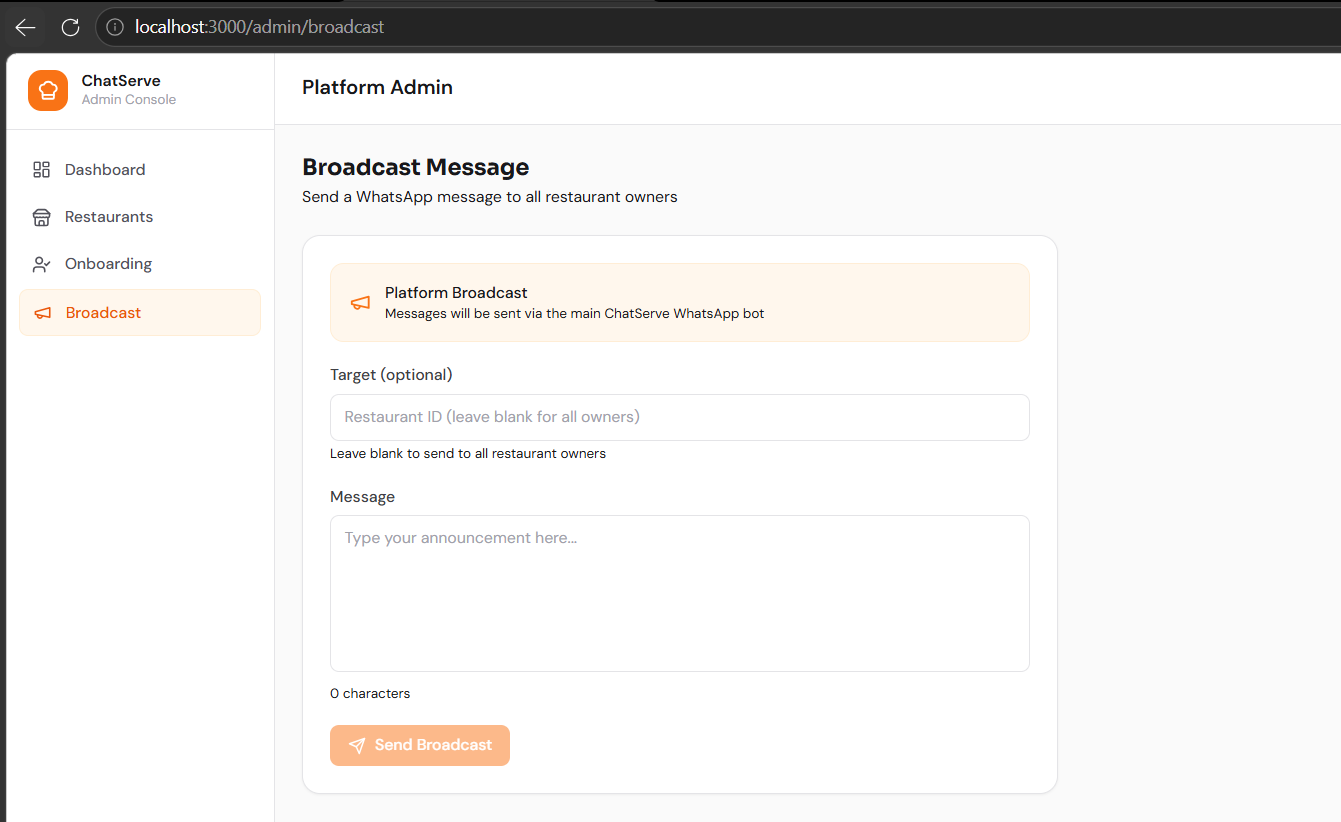
\includegraphics[width=0.95\textwidth]{Diagrams/admin_brodcast.png}
\caption{Administrator Broadcast Messaging Module}
\label{fig:admin_broadcast}
\end{figure}

The administrator can broadcast messages to all owners of registered businesses at once by using this module. The message would get sent to the owner's WhatsApp number via the Meta Cloud API.

% ── Business Owner Dashboard ───────────────────────────────────────────────
\subsection{Business Owner Dashboard}

\begin{figure}[H]
\centering
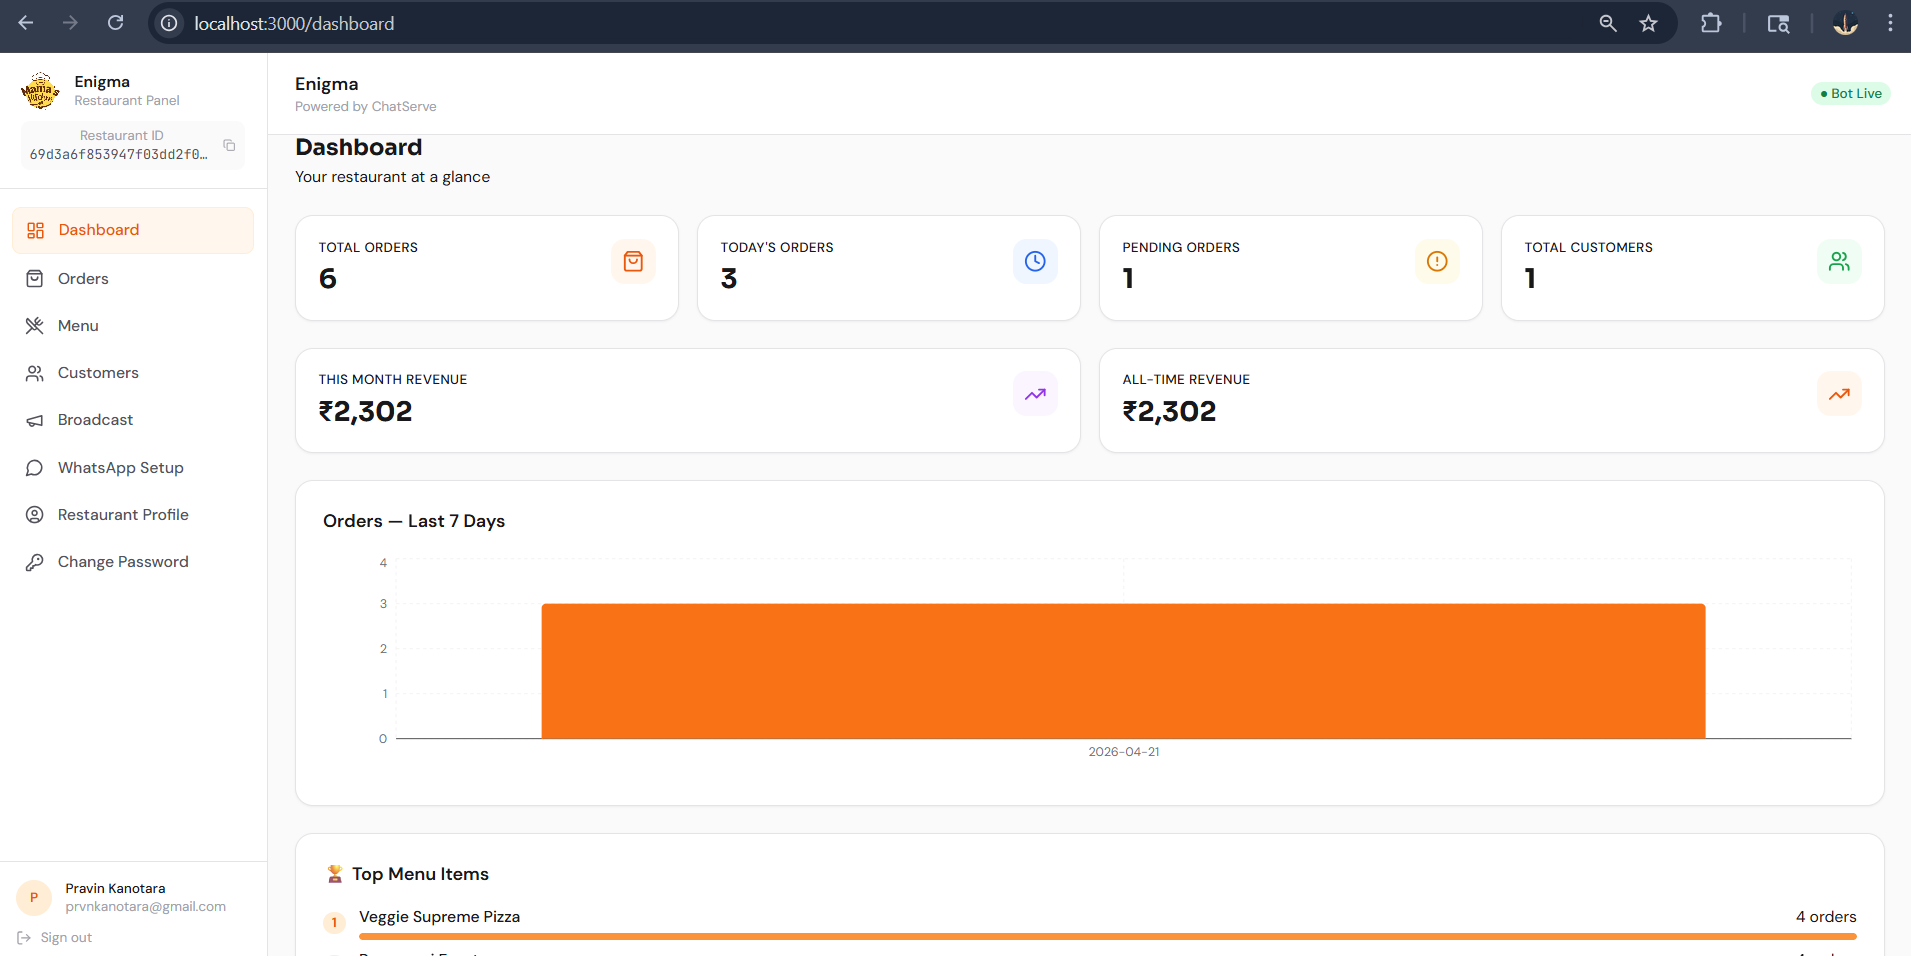
\includegraphics[width=0.95\textwidth]{Diagrams/restaurant_dashboard.png}
\caption{Business Owner Dashboard: Orders Today}
\label{fig:restaurant_dashboard}
\end{figure}

Business owners see general statistics for the day in the upper part of the screen, including the total number of orders, earned money and unique customers. Moreover, a seven-day chart showing the evolution of orders is presented here. Lastly, below that owners see the list of the orders of the day.

% ── Catalog Management ──────────────────────────────────────────────────────
\begin{figure}[H]
\centering
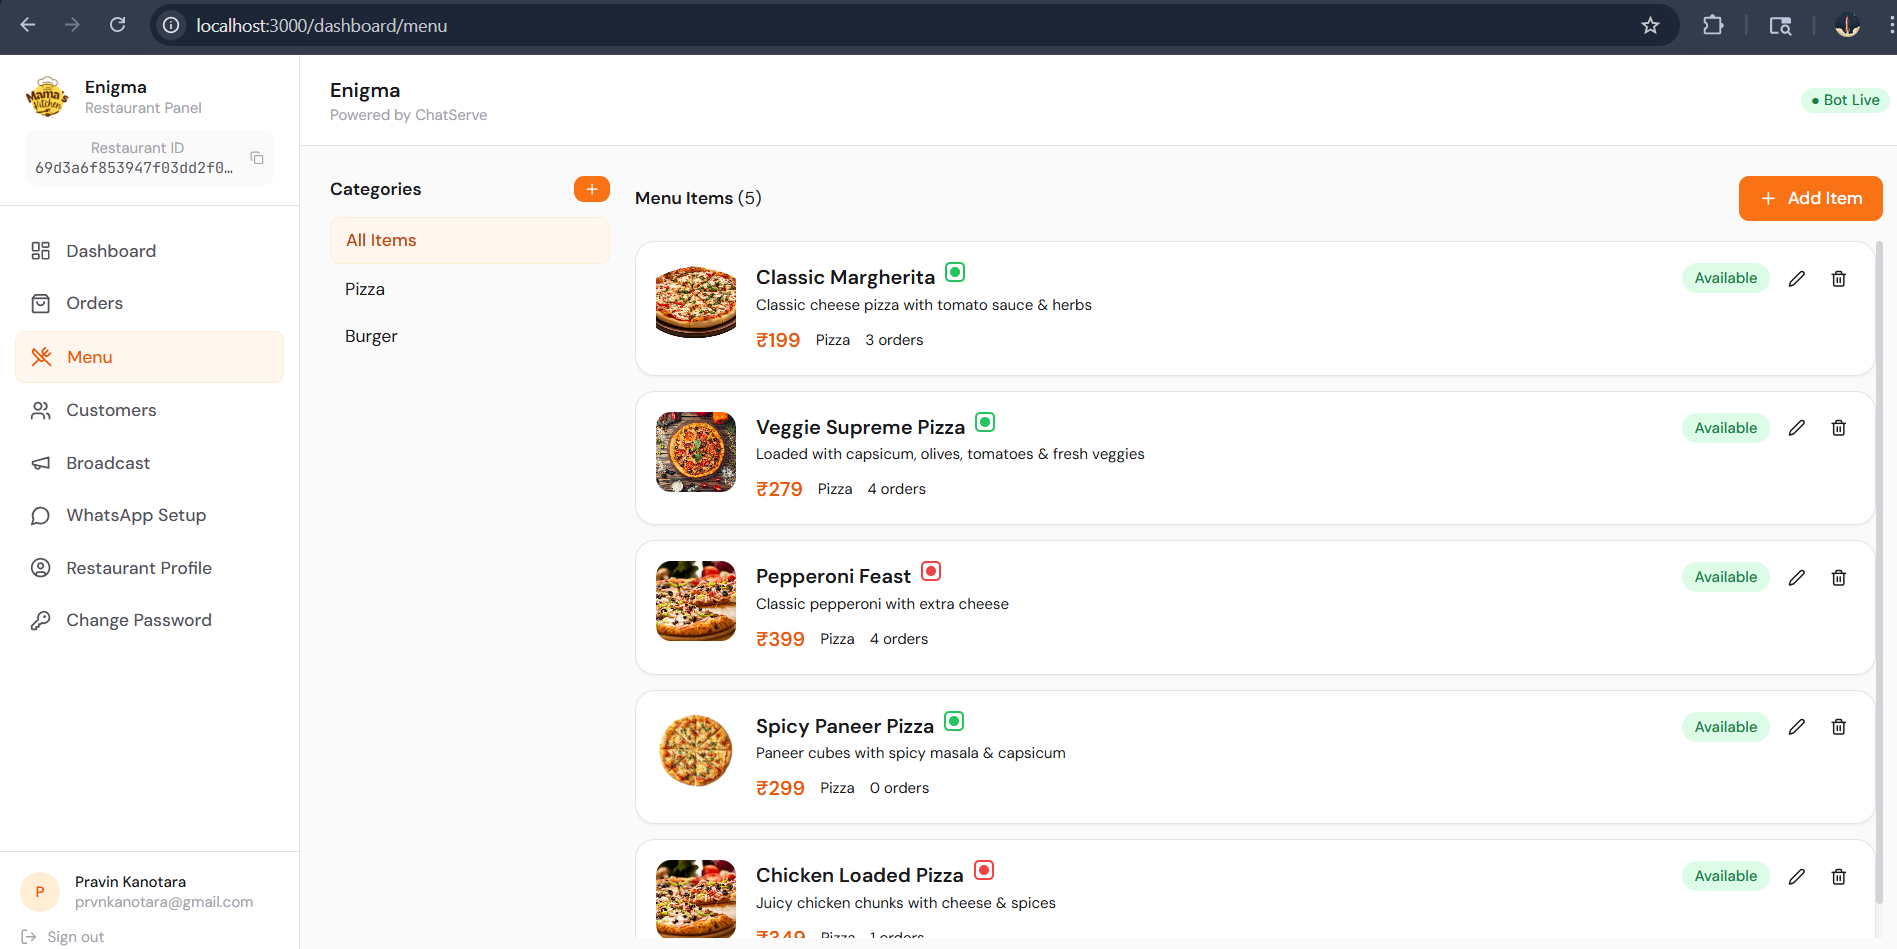
\includegraphics[width=0.95\textwidth]{Diagrams/restaurant_menu.png}
\caption{Product/Service Catalog Management Module}
\label{fig:menu_management}
\end{figure}

Catalog management allows business owners to view all products or services divided into categories. Here we can see the item name, price and status (currently active or disabled). In addition, the owner can toggle the item's status, thus changing the behavior of the bot when responding to user queries. Lastly, there is an opportunity to add new items by filling out a simple form (accessible by clicking the appropriate button).

% ── WhatsApp Business Profile ─────────────────────────────────────────────────
\begin{figure}[H]
\centering
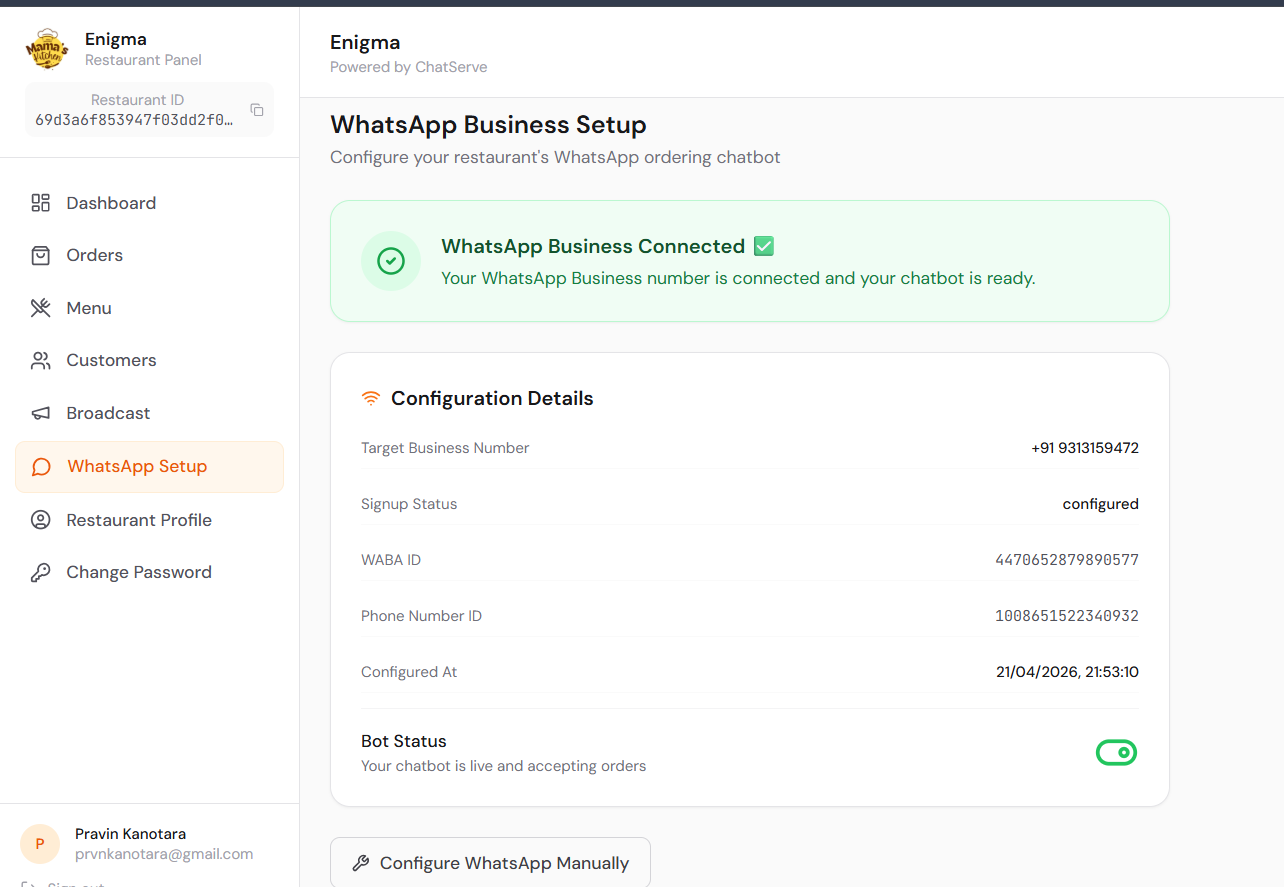
\includegraphics[width=0.85\textwidth]{Diagrams/restaurant_WAprofile.png}
\caption{Business's Auto-Configured WhatsApp Business Profile}
\label{fig:wa_profile}
\end{figure}

Below we see the automatically configured WhatsApp Business Profile of one of our businesses. It should be noted that all the data presented here was automatically populated based on the information provided by the owner during the onboarding conversation.

% ── Business Broadcast ──────────────────────────────────────────────────────
\begin{figure}[H]
\centering
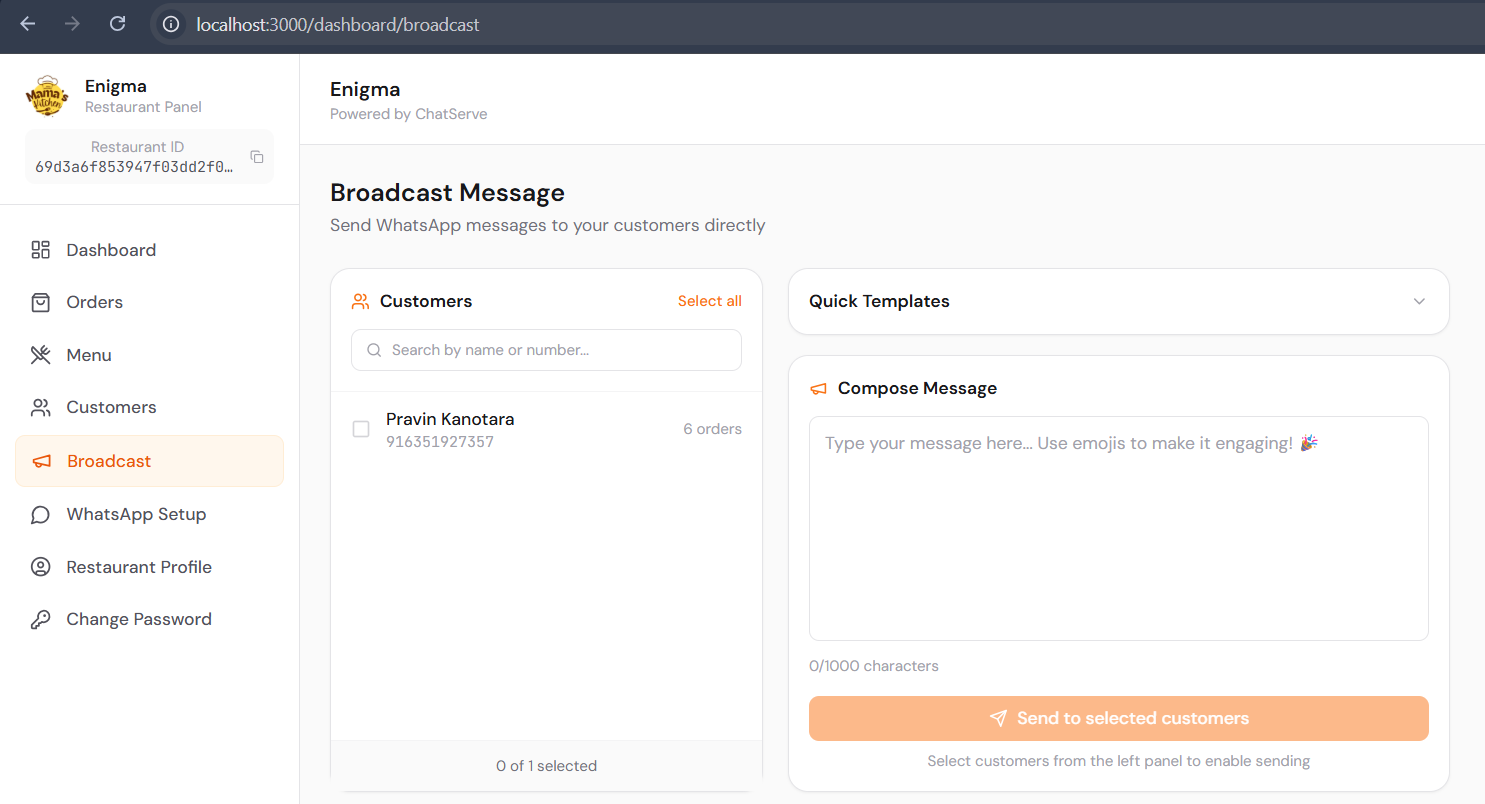
\includegraphics[width=0.95\textwidth]{Diagrams/restaurant_brodcast.png}
\caption{Business Owner's Broadcast Module}
\label{fig:restaurant_broadcast}
\end{figure}

Finally, the business owner can broadcast his own message to his customers using this module. The message would get delivered to all those customers who interacted with the business bot before.




\section{Discussion}

\subsection{Functionality Verification}

The system complies with all functional requirements, namely: business integration, WhatsApp ordering, and dashboard management. In general, the whole process of customer engagement to order confirmation works as expected.

\subsection{System Behavior}

Formal system testing could not be performed because of the lack of a production environment. But based on development and system usage, the system exhibited stable behavior for key functionalities, such as authentication, data processing, and bot messaging.

\subsection{System Design Issues}

Multi-tenant architecture allows logical data separation between different business accounts. Additionally, the system can configure automatically the WhatsApp Business Profile, including the use of the Embedded Signup feature.

Development-wise, the Manual Activation flow is used, although the system can operate fully automatically after Meta Business Verification. % Chapter 4 — Proposed Framework (all diagrams)
% ══════════════════════════════════════════════════════════════════════════════
% CHAPTER 5 — CONCLUSION AND FUTURE SCOPE
% ══════════════════════════════════════════════════════════════════════════════
\chapter{Conclusion and Future Scope}

\section{Conclusion}

To summarise, the core question of this project was whether a small business owner could access automated ordering and booking in WhatsApp Business without any prior technical knowledge or investment in cost, complexity, or dependency upon an external operator. The result provided through ChatServe is affirmative.

The major components provided include: full conversational onboarding entirely over WhatsApp, automated setup of the WABA instance using Embedded Signup, full-fledged ordering chatbot with its cart and checkout functionalities, and web-based manager's control panel --- all integrated seamlessly within the single-tenant software-as-a-service architecture to serve multiple businesses simultaneously.

The main technical contributions of this work include: production-grade multi-tenant implementation of WhatsApp SAAS functionality, complete implementation of Embedded Signup and OAuth integration with automatic post-configuration, state-machine driven dual-bot architecture, and automatic synchronization of WhatsApp Business profile from platform data. All of these components require significant effort alone, and integrating them into a coherent framework is the primary accomplishment of the work.

Finally, in terms of academic contribution, the work presents insights into the use of WhatsApp Business API as an end-to-end automation channel in developing economies --- an important commercial problem area that remains understudied in the academic community.

\section{Limitations}

Despite the successful implementation of the system, certain limitations apply due to external factors beyond the scope of development. These limitations can be grouped as follows:

\subsection{Platform and Regulatory Limitations}

\begin{itemize}
    \item Full production deployment of the Meta Embedded Signup flow requires completion of Meta Business Verification.
    \item This step is necessary to utilise production-ready WhatsApp Business API capabilities.
    \item It represents a regulatory limitation rather than any constraint related to architecture or implementation.
    \item The verification process usually includes registration of business account (e.g., Udyam MSME registration) and subsequent approval from Meta, which takes a few days.
    \item In the meantime, the system uses Manual Activation capability available through admin interface to ensure proper functioning.
\end{itemize}

\subsection{Infrastructure and Development Constraints}

\begin{itemize}
    \item Currently the system employs free tier cloud services, which come with some limitations:
    \begin{itemize}
        \item MongoDB Atlas comes with data and performance restrictions on free tier.
        \item Free tier Cloudinary imposes some storage limits.
        \item WhatsApp Business API allows only limited number of conversations per month for free.
        \item Development access tokens used temporarily expire over time, requiring periodic renewal.
    \end{itemize}
    \item None of these limitations are fundamental and can be addressed by upgrading to paid tiers.
    \item No other limitations of architectural type were encountered during development.
\end{itemize}

\section{Future Enhancements}

\subsection{Near-Future Enhancements (3--6 months)}

\begin{itemize}
    \item Implementation of Razorpay integration allowing UPI/credit/debit card payments
    \item Business verification and full production deployment of Embedded Signup
    \item Implementation of template message system to send WhatsApp messages outside 24-hour session window
\end{itemize}

\subsection{Medium-Term Enhancements (6--12 months)}

\begin{itemize}
    \item Support for several languages, e.g. Hindi, Gujarati, with automatic language detection
    \item Customer loyalty system, i.e., points collection and distribution of discount coupons
    \item Integration with WhatsApp catalogues to browse products and services
    \item NLP-based order processing, e.g. ``show me services under Rs.\ 500''
    \item Multi-platform messaging capabilities, e.g. via Instagram, Telegram, etc.
    \item Developing a mobile app for business owners
\end{itemize}

\subsection{Long-Term Enhancements (>1 year)}

\begin{itemize}
    \item Extension to additional business verticals such as healthcare providers, tutoring services, and event planners
\end{itemize}         % Chapter 5 — Conclusion and Future Scope

% ══════════════════════════════════════════════════════════════════════════════
% BACK MATTER
% ══════════════════════════════════════════════════════════════════════════════

\appendix

% ─── Appendix A — Tools and Technologies Used ────────────────────────────────
\chapter{Appendix A: Tools and Technologies Used}

\begin{table}[H]
\centering
\caption{Development Tools and Libraries}
\renewcommand{\arraystretch}{1.3}
\begin{tabularx}{\textwidth}{|l|l|X|}
\hline
\textbf{Tool / Library} & \textbf{Version} & \textbf{Purpose} \\
\hline
Node.js & 20.20.0 & Backend JavaScript runtime \\
\hline
Express.js & 4.19.2 & Web framework and API routing \\
\hline
MongoDB & 7.x & Primary NoSQL document database \\
\hline
Mongoose & 8.4.3 & MongoDB ODM with schema validation \\
\hline
React & 18.3.1 & Frontend SPA framework \\
\hline
Vite & 5.4.21 & Frontend build tool \\
\hline
Tailwind CSS & 3.4.4 & Utility-first CSS framework \\
\hline
TanStack Query & 5.45.1 & Server state management and caching \\
\hline
Axios & 1.7.2 & HTTP client with request interceptors \\
\hline
jsonwebtoken & 9.0.2 & JWT creation and verification \\
\hline
bcryptjs & 2.4.3 & Password hashing (salt factor 12) \\
\hline
Cloudinary SDK & 1.41.3 & Image upload and CDN management \\
\hline
multer-storage-cloudinary & 4.0.0 & Multipart form image upload \\
\hline
winston & 3.13.0 & Structured application logging \\
\hline
recharts & 2.12.7 & React chart components \\
\hline
react-hot-toast & 2.4.1 & In-app toast notifications \\
\hline
nodemon & 3.1.4 & Development auto-restart \\
\hline
Visual Studio Code & 1.90+ & Primary IDE \\
\hline
Postman & Latest & API testing and documentation \\
\hline
MongoDB Compass & Latest & Database inspection GUI \\
\hline
ngrok & 3.36.1 & Webhook tunnelling for local development \\
\hline
\end{tabularx}
\end{table}

% ─── Appendix B — Additional Material ───────────────────────────────────────
\chapter{Appendix B: Additional Material}


\section{Environment Configuration}

\begin{lstlisting}[caption=.env Configuration Reference (Sensitive values redacted)]
# Server
PORT=5000
NODE_ENV=development

# MongoDB
MONGODB_URI=mongodb://localhost:27017/chatserve

# JWT
JWT_ACCESS_SECRET=<32+ char random string>
JWT_REFRESH_SECRET=<32+ char random string>
JWT_ACCESS_EXPIRES=15m
JWT_REFRESH_EXPIRES=7d

# Cloudinary
CLOUDINARY_CLOUD_NAME=<cloud-name>
CLOUDINARY_API_KEY=<api-key>
CLOUDINARY_API_SECRET=<api-secret>

# Meta / WhatsApp Cloud API
META_APP_ID=<meta-app-id>
META_APP_SECRET=<meta-app-secret>
META_WEBHOOK_VERIFY_TOKEN=<random-string>
META_GRAPH_API_VERSION=v19.0

# Platform Bot Number (Test Number)
MAIN_PHONE_NUMBER_ID=<phone-number-id>
MAIN_WABA_ID=<waba-id>
MAIN_ACCESS_TOKEN=<temporary-or-permanent-token>

# Embedded Signup
META_CONFIG_ID=<embedded-signup-config-id>
EMBEDDED_SIGNUP_REDIRECT_URI=https://yourdomain/api/embedded-signup/callback

# Application URLs
FRONTEND_URL=http://localhost:3000
WEBHOOK_BASE_URL=https://yourngrok.ngrok-free.app
\end{lstlisting}

% ─── References ──────────────────────────────────────────────────────────────
\newpage
\begin{thebibliography}{99}

\bibitem{meta_cloud_api}
Meta Platforms Inc.,
``WhatsApp Cloud API Documentation,''
[Online]. Available: \url{https://developers.facebook.com/docs/whatsapp/cloud-api}

\bibitem{meta_webhooks}
Meta Platforms Inc.,
``WhatsApp Webhooks Documentation,''
[Online]. Available: \url{https://developers.facebook.com/docs/whatsapp/cloud-api/webhooks}

\bibitem{meta_messages_api}
Meta Platforms Inc.,
``Sending Messages using WhatsApp Cloud API,''
[Online]. Available: \url{https://developers.facebook.com/docs/whatsapp/cloud-api/reference/messages}

\bibitem{meta_business_profile}
Meta Platforms Inc.,
``WhatsApp Business Profile API,''
[Online]. Available: \url{https://developers.facebook.com/docs/whatsapp/cloud-api/reference/whatsapp-business-profile}

\bibitem{meta_embedded_signup}
Meta Platforms Inc.,
``Embedded Signup for WhatsApp Business Platform,''
[Online]. Available: \url{https://developers.facebook.com/docs/whatsapp/embedded-signup}

\bibitem{meta_templates}
Meta Platforms Inc.,
``Message Templates (WhatsApp Business API),''
[Online]. Available: \url{https://developers.facebook.com/docs/whatsapp/message-templates}

\bibitem{meta_pricing}
Meta Platforms Inc.,
``WhatsApp Business Platform Pricing,''
[Online]. Available: \url{https://developers.facebook.com/docs/whatsapp/pricing}

\bibitem{meta_business_management}
Meta Platforms Inc.,
``WhatsApp Business Management API,''
[Online]. Available: \url{https://developers.facebook.com/docs/whatsapp/business-management-api}

\bibitem{meta_whatsapp}
Meta Platforms Inc., 
``WhatsApp Business Platform Overview,'' 
2024. [Online]. Available: \url{https://developers.facebook.com/docs/whatsapp}

\bibitem{msme_annual_report}
Ministry of Micro, Small and Medium Enterprises, Government of India, 
``Annual Report 2022--23,'' 
New Delhi, 2023. [Online]. Available: \url{https://dashboard.msme.gov.in/}

\bibitem{pib_msme2025}
Press Information Bureau. ``MSME sector accounts for 30.1\% of India's GDP, 35.4\% of manufacturing and 45.73\% of exports in the country: Union Minister for MSME.'' \textit{Ministry of Micro, Small \& Medium Enterprises}, July 4, 2025.

\bibitem{chegg_homebusiness2025}
Sharma, Anshika. ``50 Best Home Based Business Ideas for 2025 : Start Now.'' \textit{Chegg}, July 24, 2025.

\bibitem{infobip_stats2026}
Posavac, Sandra. ``WhatsApp statistics 2026: Market analysis \& global usage data.'' \textit{Infobip}, April 20, 2026.

\bibitem{hyperleap_india2026}
Lakkepuram, Gopi Krishna. ``WhatsApp Business Statistics India 2026.'' \textit{Hyperleap AI}, October 8, 2025.

\bibitem{thunderbit_stats2025}
Guan, Shuai. ``110 WhatsApp Statistics and Facts.'' \textit{Thunderbit}, December 30, 2025.

\bibitem{setter_stats2025}
Tzschetzsch, Timo. ``WhatsApp Business Statistics: 25 Stats You Can't Ignore [2025].'' \textit{Setter AI}, November 27, 2025.

\bibitem{d7_stats2026}
Kurian, Saumya. ``60 WhatsApp Business Statistics You Need to Know in 2026.'' \textit{D7 Networks}, November 11, 2024.

\bibitem{whatsapp_difference}
WhatsApp. ``The Difference Between WhatsApp and WhatsApp for Business.'' \textit{WhatsApp Official Website}.


\end{thebibliography}



% ══════════════════════════════════════════════════════════════════════════════
\end{document}
% ══════════════════════════════════════════════════════════════════════════════
